% questions.tex —— 2015 年·安徽卷·理科 · 题目内容片段（无答案）
% 由 tools/generate_projects.py 依来源总账自 2015/2015_数学真题_安徽理_试题.md 生成，勿手改（改源 MD 后重跑）


\gkpart{数学}

\begin{gktip}
\textbf{来源说明}：本题面依据固定源 PDF 全 2 页逐题核对（p1＝页 931：栏 1 标题与「一、选择题」1–7（含第 7 题三视图）；栏 2 第 8、9 题（含函数图象）与「二、填空题」11–15（含第 13 题程序框图）、「三、解答题」节头；栏 3 第 16、17 题；p2＝页 932：栏 1 第 18、19 题（含多面体图）、栏 2 第 20 题、栏 3 第 21 题）。原卷为 \textbf{A3 横向三栏书刊合排}，阅读序＝左→中→右；\textbf{页脚仅印合订本书页页码 931／932}，\textbf{无页眉}；标题在栏 1 内排印。\textbf{全卷不印分值、不印题量、不印「考生注意」栏}——三处节头逐字仅「一、选择题」「二、填空题」「三、解答题」；总分 150 为结构推断，\textbf{卷面无凭据}，本文件不作补写。

\textbf{源制作体系判定}（实测）：源\textbf{不是扫描件，而是 LaTeX（Computer Modern 系）重排产物}——\texttt{pdfimages -list} 零命中（全页无位图）；嵌入字体含中文 \textbf{STSong／STHeiti}，拉丁与数学 \textbf{LMRoman 系与 CM 系（CMR10／CMR7／CMMI10／CMMI7／CMSY10／CMSY7／CMEX10／MSAM10／CMMIB10）}，另有 \textbf{TeX-vect10}（向量长箭头）。文本层整体可读；根号上划线、分式横线、作答横线、全部箭头与向量箭杆均为矢量路径（\textbf{「$\parallel$」（第 19 题 (1)）为字体字形但无 ToUnicode 映射}，文本层完全丢失该符号）。

\textbf{标点与字样约定（实测）}：① \textbf{题号与句末}源内为半角 \texttt{.}，按全库约定写作全角「．」；② \textbf{正文句读}源内为\textbf{半角 ASCII}（\texttt{,} \texttt{.} \texttt{;} \texttt{:}）与半角圆括号，一律归一为全角「，」「：」「；」「？」「（）」（顿号、序号「①②③④⑤」为全角照源）；③ \textbf{选项标号}半角「(A)」照录；④ \textbf{作答空}：填空为统一横线（实测 \textbf{31.50 pt}＝3 em，写作 \texttt{\gkblank{}}），选择题作答括注写作「（　）」（源为半角括号＋固定 10.50 pt 空档）；⑤ \textbf{分数}均为显示风格（真分式），排印一律 \(\dfrac{a}{b}\)；⑥ \textbf{不等号}按 MSAM10 实测排 \(\geqslant\)／\(\leqslant\)（第 13、18、21 题）；⑦ \textbf{向量}：本卷\textbf{有 CMMIB10}——第 8 题的向量 \(\boldsymbol{a}\)、\(\boldsymbol{b}\) 为\textbf{粗斜体}（墨迹较常规斜体 +65\%，实测独立判定），录作 \(\boldsymbol{a}\)／\(\boldsymbol{b}\)；\(\overrightarrow{AB}\) 类为 \textbf{TeX-vect10 长箭头}照录；⑧ \textbf{正体}：\(\sin\)／\(\cos\)／\(\ln\)（LMRoman10）、虚数单位 \(\mathrm{i}\)（第 1 题）、实数集 \(\mathbf{R}\)（第 12 题，源为\textbf{粗正体} LMRoman10-Bold）；⑨ 全卷\textbf{句末不用「。」}（源体系特征）；词间空格照页面词界补。

\textbf{存疑与登记}（源内异常一律照录；完整清单见工作档 \texttt{figure-inventory.md} 与转录稿存疑表）：① \textbf{固定源不附参考答案}（等级 D）——解析全部由本库独立推导；② \textbf{第 8 题「满足」后有一处半角逗号}（与句法不符，600 dpi 复核为真逗号）——\textbf{照源保留}；③ \textbf{第 13 题判断框内为十进制 \texttt{1.414}}（非 \(\sqrt{2}\)）——照源复刻；④ 第 13 题循环\textbf{回边并入主脊}（尖端高出菱形顶 7.37 pt，非汇入菱形左顶点）——照源；⑤ \textbf{第 19 题 (1) 的「$\parallel$」}文本层丢失——按语义排印 \(\parallel\)；⑥ 第 19 题虚线棱共 4 条，含截面边 \(D\text{-}A_1\)（与「截面边用实线」惯例不同）——照源；⑦ 第 7 题三视图内有两组重复绘制的短线段（无墨迹差异）——源内冗余，登记备查；⑧ 第 16、17、21 题题号越出栏界伸入栏间空白（悬挂缩进排版本相）——照源；⑨ 第 15 题选项「①②③④」以分号结尾、⑤ 以句点结尾（源内混排）——照源；⑩ 第 9 题图象的标注字母与曲线特征点为\textbf{示意性对应}（照源复刻，不据题面反推）。
\end{gktip}

\gkpart{试题}

\gkpart{一、选择题}

\begin{question}
\gkti{1}设 \(\mathrm{i}\) 是虚数单位，则复数 \(\dfrac{2\mathrm{i}}{1-\mathrm{i}}\) 在复平面内所对应的点位于（　）

(A) 第一象限　(B) 第二象限　(C) 第三象限　(D) 第四象限

\end{question}
\begin{question}
\gkti{2}下列函数中，既是偶函数又存在零点的是（　）

(A) \(y=\cos x\)　(B) \(y=\sin x\)　(C) \(y=\ln x\)　(D) \(y=x^2+1\)

\end{question}
\begin{question}
\gkti{3}设 \(p\)：\(1<x<2\)，\(q\)：\(2^x>1\)，则 \(p\) 是 \(q\) 成立的（　）

(A) 充分不必要条件　(B) 必要不充分条件

(C) 充分必要条件　(D) 既不充分也不必要条件

\end{question}
\begin{question}
\gkti{4}下列双曲线中，焦点在 \(y\) 轴上且渐近线方程为 \(y=\pm 2x\) 的是（　）

(A) \(x^2-\dfrac{y^2}{4}=1\)　(B) \(\dfrac{x^2}{4}-y^2=1\)

(C) \(\dfrac{y^2}{4}-x^2=1\)　(D) \(y^2-\dfrac{x^2}{4}=1\)

\end{question}
\begin{question}
\gkti{5}已知 \(m\)，\(n\) 是两条不同直线，\(\alpha\)，\(\beta\) 是两个不同平面，则下列命题正确的是（　）

(A) 若 \(\alpha\)，\(\beta\) 垂直于同一平面，则 \(\alpha\) 与 \(\beta\) 平行

(B) 若 \(m\)，\(n\) 平行于同一平面，则 \(m\) 与 \(n\) 平行

(C) 若 \(\alpha\)，\(\beta\) 不平行，则在 \(\alpha\) 内不存在与 \(\beta\) 平行的直线

(D) 若 \(m\)，\(n\) 不平行，则 \(m\) 与 \(n\) 不可能垂直于同一平面

\end{question}
\begin{question}
\gkti{6}若样本数据 \(x_1\)，\(x_2\)，\(\cdots\)，\(x_{10}\) 的标准差为 8，则数据 \(2x_1-1\)，\(2x_2-1\)，\(\cdots\)，\(2x_{10}-1\) 的标准差为（　）

(A) 8　(B) 15　(C) 16　(D) 32

\Needspace{0.4\textheight}
\end{question}
\begin{question}
\gkti{7}一个四面体的三视图如图所示，则该四面体的表面积是（　）
\nopagebreak[4]
\begin{center}% ============================================================
% f2015ahl_q07_views.tex —— 2015 安徽卷（理）第 7 题 三视图与尺寸标注
%
% 【来源】工作档 .work/phase3-b13/source/2015安徽理.pdf（sha256 402eca00…ce7b0）
%          第 1 页（页脚 931）栏 1；坐标数据取自实测清单
%          .work/phase3-b13/figure-inventory.md §F01（要素表 P031–P075、箭头表、标签表）。
% 【坐标口径】真页 pt（PDF 页面坐标，原点页左下角，1190.55 × 841.89 bp）。
%          画布 1 单位 = 1 TeX pt，图内坐标直接写字面值（清单已给真页 pt）。
%          清单 §0.3 本卷实测换算因子 a_x = 0.999622795、a_y = 0.999621571，
%          与 1 的偏差 3.8e-4 系渲染器取整所致（非页面缩放），故不再二次缩放。
%          注：1 TeX pt = 0.996264 bp，故本图绝对尺寸比源件小 0.375%（项目定型口径）。
% 【线宽】0.3980 pt：3 个三角形三边、2 条高、12 条尺寸线本体、10 条竖刻度、
%          14 条 √2 引线（本体+刻度）；0.4200 pt：4 处「√2」根号上横线。
%          注：清单 §F01.2(c) 小标题写「尺寸线本体 lw = 0.42 pt」，与其 §F01.2 末尾
%          「线宽分档」表（0.398 × 45 + 0.42 × 4）及源件实测（P007…P029 全为 0.3980）
%          矛盾 —— 此处按源件实测与分档表取 0.3980，仅 4 条根号上横线为 0.4200。
% 【照源复刻的存疑项】
%   1) 源件中俯视图右侧两条 √2 引线刻度被重绘一次（P070/P071 与 P056/P057 端点逐位
%      相同，清单 FI-S1）—— 几何重合，此处只画一次。
%   2) 4 处「√2」的根号上横线（P072–P075，lw 0.42）不另画路径：本图用 `$\sqrt{2}$`
%      排版，横线由 TeX 根号构造内生（与源件同构，源件亦为 CMSY10 根号 + 独立横线）。
%   3) 三视图形「底宽 2、高 1」与侧视图「1 × 1」的几何基准不统一（FI-S15），
%      照源复刻不改。
%   4) 标签按【源墨迹实测中心】放置；清单给的是 pdftohtml em 框中心（西文含 descend，
%      中心偏低约 1.3–1.5 pt；CMSY10 根号框另有上偏），故坐标 = 清单值 + 墨迹修正。
%   5) 「正(主)视图」等中文标签用半角括号直排（源件括号为 LMRoman10 半角），
%      中西文间距由 ctex 默认 CJKecglue 生成，与源件的间距可能略有差异。
% ============================================================
% 【自验】（探针 .work/phase3-b13/probe/q07-probe.tex，latexmk -pdfxe）
%   编译：0 error、0 Overfull、0 Underfull、0 Missing character。
%   字面量反算双层核对（A 手工誊录清单字面量 + B 源 PDF 逐命令复解析，含两条
%   曲线的全部 598 段控制点）：最大残差 0.0005 pt（阈值 0.05）。
%   600 dpi 墨迹核对（源件页 vs 探针对位后）：几何 345 点采样 max 0.145 pt / rms 0.109 pt，标签墨迹质心 max 0.127 pt；
%   并排与红蓝重合裁片见 probe/crops/q07-side.png、q07-overlay.png。
\begin{tikzpicture}[x=1pt, y=1pt,
    every node/.style={font=\fontsize{10.5pt}{12.6pt}\selectfont, inner sep=0pt}]
  \begin{scope}[line width=0.398pt]
    % ---------- 三角形与高（清单 §F01.2(a)）----------
    \draw (135.701,215.511) -- (223.009,215.511) -- (179.355,259.165) -- cycle;  % P044 正视图
    \draw (179.355,215.511) -- (179.355,259.165);                                % P043 正视图高
    \draw (135.701,150.030) -- (223.009,150.030) -- (179.355,106.376) -- cycle;  % P041 俯视图
    \draw (179.355,150.030) -- (179.355,106.376);                                % P042 俯视图高
    \draw (266.663,215.511) -- (310.317,215.511) -- (266.663,259.165) -- cycle;  % P045 侧视图
    % ---------- 尺寸刻度线（§F01.2(b)，10 条）----------
    \draw (135.701,154.396) -- (135.701,163.127);   % P036 俯视图行左
    \draw (179.355,154.396) -- (179.355,163.127);   % P037 俯视图行中
    \draw (223.009,154.396) -- (223.009,163.127);   % P038 俯视图行右
    \draw (135.701,202.414) -- (135.701,211.145);   % P033 正视图行左
    \draw (179.355,202.414) -- (179.355,211.145);   % P034 正视图行中
    \draw (223.009,202.414) -- (223.009,211.145);   % P035 正视图行右
    \draw (266.663,202.414) -- (266.663,211.145);   % P039 侧视图行左
    \draw (310.317,202.414) -- (310.317,211.145);   % P040 侧视图行右
    \draw (253.566,215.511) -- (262.297,215.511);   % P031 侧视图竖标下
    \draw (253.566,259.165) -- (262.297,259.165);   % P032 侧视图竖标上
    % ---------- 尺寸线本体（§F01.2(c)，12 条）----------
    \draw (139.2872,158.7605) -- (148.7972,158.7605);   % P007 俯视图左段
    \draw (166.2585,158.7605) -- (175.7685,158.7605);   % P009 俯视图左段尾
    \draw (182.9411,158.7605) -- (192.4511,158.7605);   % P011 俯视图右段首
    \draw (209.9124,158.7605) -- (219.4224,158.7605);   % P013 俯视图右段
    \draw (139.2872,206.7800) -- (148.7972,206.7800);   % P015 正视图左段
    \draw (166.2585,206.7800) -- (175.7685,206.7800);   % P017 正视图左段尾
    \draw (182.9411,206.7800) -- (192.4511,206.7800);   % P019 正视图右段首
    \draw (209.9124,206.7800) -- (219.4224,206.7800);   % P021 正视图右段
    \draw (270.2489,206.7800) -- (279.7589,206.7800);   % P023 侧视图横标左
    \draw (297.2202,206.7800) -- (306.7302,206.7800);   % P025 侧视图横标右
    \draw (257.9320,219.0970) -- (257.9320,228.6070);   % P027 侧视图竖标上
    \draw (257.9320,246.0680) -- (257.9320,255.5780);   % P029 侧视图竖标下
    % ---------- √2 引线与刻度（§F01.2(c)，P070/P071 与 P056/P057 重合故略）----------
    \draw (133.518,147.847) -- (126.533,140.862);   % P046 俯视图左刻度
    \draw (177.172,104.193) -- (170.187,97.208);    % P047 俯视图左刻度（下）
    \draw (143.122,131.258) -- (132.562,141.818);   % P048 俯视图左引线本体
    \draw (160.583,113.797) -- (171.143,103.237);   % P050 俯视图左引线本体
    \draw (215.588,131.258) -- (226.148,141.818);   % P052 俯视图右引线本体
    \draw (198.126,113.797) -- (187.566,103.237);   % P054 俯视图右引线本体
    \draw (225.191,147.847) -- (232.177,140.862);   % P056 俯视图右刻度
    \draw (181.538,104.193) -- (188.523,97.208);    % P057 俯视图右刻度（下）
    \draw (133.518,217.694) -- (126.533,224.679);   % P058 正视图左刻度
    \draw (177.172,261.347) -- (170.187,268.332);   % P059 正视图左刻度（上）
    \draw (225.191,217.694) -- (232.177,224.679);   % P060 正视图右刻度
    \draw (181.538,261.347) -- (188.523,268.332);   % P061 正视图右刻度（上）
    \draw (143.122,234.282) -- (132.562,223.722);   % P062 正视图左引线本体
    \draw (160.583,251.744) -- (171.143,262.303);   % P064 正视图左引线本体
    \draw (215.588,234.282) -- (226.148,223.722);   % P066 正视图右引线本体
    \draw (198.126,251.744) -- (187.566,262.303);   % P068 正视图右引线本体
    % ---------- 20 个填充箭头（尖端坐标取清单；Triangle 长 3.985 / 宽 2.988）----------
    \draw[{Triangle[length=3.985pt,width=2.988pt]}-] (135.7009,158.7605) -- (139.6859,158.7605);  % P008 ← 俯视图左端
    \draw[{Triangle[length=3.985pt,width=2.988pt]}-] (179.3547,158.7605) -- (175.3697,158.7605);  % P010 → 俯视图中点
    \draw[{Triangle[length=3.985pt,width=2.988pt]}-] (179.3548,158.7605) -- (183.3398,158.7605);  % P012 ← 俯视图中点
    \draw[{Triangle[length=3.985pt,width=2.988pt]}-] (223.0086,158.7605) -- (219.0236,158.7605);  % P014 → 俯视图右端
    \draw[{Triangle[length=3.985pt,width=2.988pt]}-] (135.7009,206.7800) -- (139.6859,206.7800);  % P016 ← 正视图左端
    \draw[{Triangle[length=3.985pt,width=2.988pt]}-] (179.3547,206.7800) -- (175.3697,206.7800);  % P018 → 正视图中点
    \draw[{Triangle[length=3.985pt,width=2.988pt]}-] (179.3548,206.7800) -- (183.3398,206.7800);  % P020 ← 正视图中点
    \draw[{Triangle[length=3.985pt,width=2.988pt]}-] (223.0086,206.7800) -- (219.0236,206.7800);  % P022 → 正视图右端
    \draw[{Triangle[length=3.985pt,width=2.988pt]}-] (266.6626,206.7800) -- (270.6476,206.7800);  % P024 ← 侧视图左端
    \draw[{Triangle[length=3.985pt,width=2.988pt]}-] (310.3164,206.7800) -- (306.3314,206.7800);  % P026 → 侧视图右端
    \draw[{Triangle[length=3.985pt,width=2.988pt]}-] (257.9319,215.5107) -- (257.9319,219.4957);  % P028 ↓ 侧视图竖标下端
    \draw[{Triangle[length=3.985pt,width=2.988pt]}-] (257.9319,259.1645) -- (257.9319,255.1795);  % P030 ↑ 侧视图竖标上端
    \draw[{Triangle[length=3.985pt,width=2.988pt]}-] (130.0257,144.3546) -- (132.8436,141.5368);  % P049 ↖ 俯视图左 √2 上端
    \draw[{Triangle[length=3.985pt,width=2.988pt]}-] (173.6795,100.7008) -- (170.8616,103.5186);  % P051 ↘ 俯视图左 √2 下端
    \draw[{Triangle[length=3.985pt,width=2.988pt]}-] (228.6838,144.3546) -- (225.8660,141.5368);  % P053 ↗ 俯视图右 √2 上端
    \draw[{Triangle[length=3.985pt,width=2.988pt]}-] (185.0300,100.7008) -- (187.8479,103.5186);  % P055 ↙ 俯视图右 √2 下端
    \draw[{Triangle[length=3.985pt,width=2.988pt]}-] (130.0257,221.1859) -- (132.8436,224.0037);  % P063 ↖ 正视图左 √2 上端
    \draw[{Triangle[length=3.985pt,width=2.988pt]}-] (173.6795,264.8397) -- (170.8616,262.0219);  % P065 ↗ 正视图左 √2 下端
    \draw[{Triangle[length=3.985pt,width=2.988pt]}-] (228.6838,221.1859) -- (225.8660,224.0037);  % P067 ↗ 正视图右 √2 上端
    \draw[{Triangle[length=3.985pt,width=2.988pt]}-] (185.0300,264.8397) -- (187.8479,262.0219);  % P069 ↙ 正视图右 √2 下端
  \end{scope}
  % ---------- 文字标签（源墨迹实测中心；行末为清单 em 框中心，供追溯）----------
  \node at (146.621,121.640) {$\sqrt{2}$};   % L q07_sqrt2_tl  √(143.733,129.419) 2(151.403,119.412)
  \node at (206.007,121.076) {$\sqrt{2}$};   % L q07_sqrt2_tr  √(203.094,129.419) 2(210.097,119.412)
  \node at (157.485,206.699) {$1$};          % L q07_1_fl      (157.406,205.469)
  \node at (201.120,206.699) {$1$};          % L q07_1_fr      (201.426,205.469)
  \node at (157.492,158.792) {$1$};          % L q07_1_tl      (157.406,157.437)
  \node at (201.137,158.742) {$1$};          % L q07_1_tr      (201.426,157.437)
  \node at (288.506,206.699) {$1$};          % L q07_1_side_h  (288.800,205.469)
  \node at (257.938,237.218) {$1$};          % L q07_1_side_v  (258.119,236.156)
  \node at (179.108,184.927) {正(主)视图};    % L q07_front     核字框并集 x[150.736,208.096] y[179.452,190.793]
  \node at (288.329,184.825) {侧(左)视图};    % L q07_side      核字框并集 x[260.120,317.480] y[179.452,190.793]
  \node at (179.389,84.540) {俯视图};         % L q07_top       (179.083,84.723)
  \node at (146.725,243.978) {$\sqrt{2}$};   % L q07_sqrt2_fl  √(143.733,251.500) 2(151.403,242.160)
  \node at (206.132,244.216) {$\sqrt{2}$};   % L q07_sqrt2_fr  √(203.094,251.500) 2(210.097,242.160)
\end{tikzpicture}
\end{center}
\nopagebreak[4]
(A) \(1+\sqrt{3}\)　(B) \(2+\sqrt{3}\)　(C) \(1+2\sqrt{2}\)　(D) \(2\sqrt{2}\)

\end{question}
\begin{question}
\gkti{8}\(\triangle ABC\) 是边长为 2 的等边三角形，已知向量 \(\boldsymbol{a}\)，\(\boldsymbol{b}\) 满足，\(\overrightarrow{AB}=2\boldsymbol{a}\)，\(\overrightarrow{AC}=2\boldsymbol{a}+\boldsymbol{b}\)，则下列结论正确的是（　）

(A) \(|\boldsymbol{b}|=1\)　(B) \(\boldsymbol{a}\perp\boldsymbol{b}\)

(C) \(\boldsymbol{a}\cdot\boldsymbol{b}=1\)　(D) \((4\boldsymbol{a}+\boldsymbol{b})\perp\overrightarrow{BC}\)

\Needspace{0.4\textheight}
\end{question}
\begin{question}
\gkti{9}函数 \(f(x)=\dfrac{ax+b}{(x+c)^2}\) 的图象如图所示，则下列结论成立的是（　）
\nopagebreak[4]
\begin{center}% ============================================================
% f2015ahl_q09_graph.tex —— 2015 安徽卷（理）第 9 题 函数图象
%
% 【来源】工作档 .work/phase3-b13/source/2015安徽理.pdf（sha256 402eca00…ce7b0）
%          第 1 页（页脚 931）栏 2；坐标数据取自实测清单
%          .work/phase3-b13/figure-inventory.md §F02（要素表 P081–P087、曲线判定 §F02.3、
%          标签表 §F02.4）。
% 【坐标口径】真页 pt（PDF 页面坐标，原点页左下角，1190.55 × 841.89 bp）。
%          画布 1 单位 = 1 TeX pt，图内坐标直接写字面值（清单已给真页 pt）。
%          清单 §0.3 本卷实测换算因子 a_x = 0.999622795、a_y = 0.999621571，
%          与 1 的偏差 3.8e-4 系渲染器取整所致（非页面缩放），故不再二次缩放。
%          注：1 TeX pt = 0.996264 bp，故本图绝对尺寸比源件小 0.375%（项目定型口径）。
% 【线宽】轴与竖直渐近线 0.3980 pt；两条曲线 0.7970 pt（全卷最粗档）。
% 【虚线】竖直渐近线 dash pattern on/off 各 2.989 pt（源件声明 `[2.989 2.989] 0 d`）。
% 【曲线复刻】两支曲线均为【贝塞尔折链】：各 m×1 + c×299（共 299 段三次贝塞尔，
%          清单 §F02.3），**非圆弧**（控制点/弦长比跨度 0.26–0.74，非恒 κ=0.5523）、
%          **非折线**（无连续 l 段）。此处按段照录为 `.. controls (c1) and (c2) ..`，
%          与源件逐控制点一致（每段 6 个坐标字面值）。
%          左支末段（(588.5346,596.4705) → (588.6936,589.0535)）源件为 c1 = c2 的退化段，
%          照录不修饰。
% 【照源复刻的存疑项】
%   1) y 轴箭头【不在轴线末端】：箭头在轴线顶端之外再高出 3.586 pt（清单 FI-S3），
%      尖端 y = 671.9526 而轴线止于 668.3663 —— 照源保留。
%   2) 竖直虚线与曲线不接触：左支最右端 x = 588.6936 与渐近线 x = 592.1251 间隙
%      3.4315 pt（FI-S6），照源保留。
%   3) M/N/O/P 四个标注与曲线／轴线的解析特征逐一对不上（O 落在 y 轴左侧 7.86 pt、
%      N 在 x 轴下方、P 落在渐近线右侧 4.94 pt，FI-S7）—— 标注位置一律照清单实测坐标
%      复刻（示意性对应），不据题面反推、不「修正」。
%   4) 「N」「P」在源件文本层被并为单个运行 `N P`（FI-S4），二者中心由 600 dpi 墨迹
%      实测拆开给出（N = 580.740、P = 597.780），精度优于清单的目视估读（±1 pt）。
%   5) 标签按【源墨迹实测中心】放置；清单给的是 pdftohtml em 框中心（CMMI10 含 descend，
%      中心偏低约 1.0 pt），故坐标 = 清单值 + 墨迹修正。
% ============================================================
% 【自验】（探针 .work/phase3-b13/probe/q09-probe.tex，latexmk -pdfxe）
%   编译：0 error、0 Overfull、0 Underfull、0 Missing character。
%   字面量反算双层核对（A 手工誊录清单字面量 + B 源 PDF 逐命令复解析，含两条
%   曲线的全部 598 段控制点）：最大残差 0.0015 pt（阈值 0.05）。
%   600 dpi 墨迹核对（源件页 vs 探针对位后）：几何 1821 点采样 max 0.127 pt / rms 0.063 pt，标签墨迹质心 max 0.136 pt；
%   并排与红蓝重合裁片见 probe/crops/q09-side.png、q09-overlay.png。
\begin{tikzpicture}[x=1pt, y=1pt,
    every node/.style={font=\fontsize{10.5pt}{12.6pt}\selectfont, inner sep=0pt}]
  \begin{scope}[line width=0.398pt]
    \draw (535.4324,637.9370) -- (645.2314,637.9370);   % P081 x 轴
    \draw (569.4480,581.2443) -- (569.4480,668.3663);   % P083 y 轴
    \draw[dash pattern=on 2.989pt off 2.989pt]
          (592.1251,586.9136) -- (592.1251,666.2836);   % P085 竖直渐近线（虚线）
    \draw[{Triangle[length=3.985pt,width=2.988pt]}-] (648.8178,637.9370) -- (644.8328,637.9370);  % P082 x 轴箭头
    \draw[{Triangle[length=3.985pt,width=2.988pt]}-] (569.4480,671.9526) -- (569.4480,667.9676);  % P084 y 轴箭头
  \end{scope}
  % ---------- 两条函数曲线（各 299 段三次贝塞尔，逐控制点照录）----------
  \begin{scope}[line width=0.797pt]
    \draw   % P086 左支（含极大值；末段为 c1 = c2 退化段）
  (541.1016,642.4165)
    .. controls (541.1016,642.4165) and (541.2166,642.4255) .. (541.2606,642.4285)
    .. controls (541.3046,642.4315) and (541.3756,642.4375) .. (541.4196,642.4405)
    .. controls (541.4636,642.4445) and (541.5346,642.4495) .. (541.5796,642.4535)
    .. controls (541.6236,642.4565) and (541.6946,642.4625) .. (541.7386,642.4655)
    .. controls (541.7826,642.4695) and (541.8536,642.4745) .. (541.8976,642.4785)
    .. controls (541.9416,642.4815) and (542.0126,642.4875) .. (542.0566,642.4905)
    .. controls (542.1006,642.4945) and (542.1716,642.5005) .. (542.2156,642.5035)
    .. controls (542.2596,642.5075) and (542.3306,642.5125) .. (542.3746,642.5165)
    .. controls (542.4196,642.5195) and (542.4896,642.5255) .. (542.5346,642.5295)
    .. controls (542.5786,642.5325) and (542.6496,642.5385) .. (542.6936,642.5425)
    .. controls (542.7376,642.5455) and (542.8086,642.5515) .. (542.8526,642.5555)
    .. controls (542.8966,642.5585) and (542.9676,642.5645) .. (543.0116,642.5685)
    .. controls (543.0556,642.5715) and (543.1266,642.5775) .. (543.1706,642.5815)
    .. controls (543.2146,642.5845) and (543.2856,642.5905) .. (543.3296,642.5945)
    .. controls (543.3746,642.5975) and (543.4446,642.6035) .. (543.4896,642.6075)
    .. controls (543.5336,642.6105) and (543.6046,642.6175) .. (543.6486,642.6205)
    .. controls (543.6926,642.6245) and (543.7636,642.6305) .. (543.8076,642.6345)
    .. controls (543.8516,642.6375) and (543.9226,642.6435) .. (543.9666,642.6475)
    .. controls (544.0106,642.6515) and (544.0816,642.6575) .. (544.1256,642.6615)
    .. controls (544.1696,642.6645) and (544.2406,642.6715) .. (544.2846,642.6745)
    .. controls (544.3296,642.6785) and (544.3996,642.6845) .. (544.4446,642.6885)
    .. controls (544.4886,642.6925) and (544.5596,642.6985) .. (544.6036,642.7025)
    .. controls (544.6476,642.7065) and (544.7186,642.7125) .. (544.7626,642.7165)
    .. controls (544.8066,642.7195) and (544.8776,642.7265) .. (544.9216,642.7295)
    .. controls (544.9656,642.7335) and (545.0366,642.7405) .. (545.0806,642.7445)
    .. controls (545.1246,642.7475) and (545.1956,642.7545) .. (545.2396,642.7585)
    .. controls (545.2846,642.7615) and (545.3546,642.7685) .. (545.3996,642.7725)
    .. controls (545.4436,642.7765) and (545.5146,642.7825) .. (545.5586,642.7865)
    .. controls (545.6026,642.7905) and (545.6736,642.7965) .. (545.7176,642.8005)
    .. controls (545.7616,642.8045) and (545.8326,642.8115) .. (545.8766,642.8155)
    .. controls (545.9206,642.8195) and (545.9916,642.8255) .. (546.0356,642.8295)
    .. controls (546.0796,642.8335) and (546.1506,642.8405) .. (546.1946,642.8445)
    .. controls (546.2396,642.8485) and (546.3096,642.8545) .. (546.3546,642.8585)
    .. controls (546.3986,642.8625) and (546.4696,642.8695) .. (546.5136,642.8735)
    .. controls (546.5576,642.8775) and (546.6286,642.8845) .. (546.6726,642.8885)
    .. controls (546.7166,642.8925) and (546.7876,642.8995) .. (546.8316,642.9035)
    .. controls (546.8756,642.9075) and (546.9466,642.9145) .. (546.9906,642.9185)
    .. controls (547.0356,642.9225) and (547.1056,642.9295) .. (547.1506,642.9335)
    .. controls (547.1946,642.9375) and (547.2656,642.9445) .. (547.3096,642.9485)
    .. controls (547.3536,642.9525) and (547.4246,642.9595) .. (547.4686,642.9635)
    .. controls (547.5126,642.9675) and (547.5836,642.9755) .. (547.6276,642.9795)
    .. controls (547.6716,642.9835) and (547.7426,642.9905) .. (547.7866,642.9945)
    .. controls (547.8306,642.9985) and (547.9016,643.0055) .. (547.9456,643.0105)
    .. controls (547.9906,643.0145) and (548.0606,643.0215) .. (548.1056,643.0255)
    .. controls (548.1496,643.0305) and (548.2206,643.0375) .. (548.2646,643.0415)
    .. controls (548.3086,643.0455) and (548.3796,643.0525) .. (548.4236,643.0575)
    .. controls (548.4676,643.0615) and (548.5386,643.0685) .. (548.5826,643.0735)
    .. controls (548.6266,643.0775) and (548.6976,643.0845) .. (548.7416,643.0895)
    .. controls (548.7856,643.0935) and (548.8566,643.1005) .. (548.9006,643.1055)
    .. controls (548.9456,643.1095) and (549.0156,643.1175) .. (549.0606,643.1215)
    .. controls (549.1046,643.1265) and (549.1756,643.1335) .. (549.2196,643.1385)
    .. controls (549.2636,643.1425) and (549.3346,643.1495) .. (549.3786,643.1545)
    .. controls (549.4226,643.1585) and (549.4936,643.1665) .. (549.5376,643.1705)
    .. controls (549.5816,643.1755) and (549.6526,643.1825) .. (549.6966,643.1875)
    .. controls (549.7406,643.1925) and (549.8116,643.1995) .. (549.8556,643.2045)
    .. controls (549.9006,643.2085) and (549.9706,643.2165) .. (550.0156,643.2205)
    .. controls (550.0596,643.2255) and (550.1306,643.2335) .. (550.1746,643.2375)
    .. controls (550.2186,643.2425) and (550.2896,643.2505) .. (550.3336,643.2545)
    .. controls (550.3776,643.2595) and (550.4486,643.2675) .. (550.4926,643.2725)
    .. controls (550.5366,643.2765) and (550.6076,643.2845) .. (550.6516,643.2895)
    .. controls (550.6956,643.2945) and (550.7666,643.3015) .. (550.8106,643.3065)
    .. controls (550.8556,643.3115) and (550.9256,643.3195) .. (550.9706,643.3245)
    .. controls (551.0146,643.3285) and (551.0856,643.3365) .. (551.1296,643.3415)
    .. controls (551.1736,643.3465) and (551.2446,643.3545) .. (551.2886,643.3595)
    .. controls (551.3326,643.3645) and (551.4036,643.3725) .. (551.4476,643.3775)
    .. controls (551.4916,643.3815) and (551.5626,643.3895) .. (551.6066,643.3945)
    .. controls (551.6506,643.3995) and (551.7216,643.4085) .. (551.7656,643.4135)
    .. controls (551.8106,643.4185) and (551.8816,643.4255) .. (551.9256,643.4315)
    .. controls (551.9696,643.4365) and (552.0406,643.4445) .. (552.0846,643.4495)
    .. controls (552.1286,643.4545) and (552.1996,643.4625) .. (552.2436,643.4675)
    .. controls (552.2876,643.4725) and (552.3586,643.4815) .. (552.4026,643.4865)
    .. controls (552.4466,643.4915) and (552.5176,643.4995) .. (552.5616,643.5045)
    .. controls (552.6066,643.5095) and (552.6766,643.5185) .. (552.7216,643.5235)
    .. controls (552.7656,643.5285) and (552.8366,643.5375) .. (552.8806,643.5425)
    .. controls (552.9246,643.5475) and (552.9956,643.5555) .. (553.0396,643.5615)
    .. controls (553.0836,643.5665) and (553.1546,643.5755) .. (553.1986,643.5805)
    .. controls (553.2426,643.5855) and (553.3136,643.5945) .. (553.3576,643.5995)
    .. controls (553.4016,643.6045) and (553.4726,643.6135) .. (553.5166,643.6185)
    .. controls (553.5616,643.6245) and (553.6316,643.6325) .. (553.6766,643.6385)
    .. controls (553.7206,643.6435) and (553.7916,643.6525) .. (553.8356,643.6585)
    .. controls (553.8796,643.6635) and (553.9506,643.6725) .. (553.9946,643.6775)
    .. controls (554.0386,643.6835) and (554.1096,643.6925) .. (554.1536,643.6975)
    .. controls (554.1976,643.7035) and (554.2686,643.7115) .. (554.3126,643.7175)
    .. controls (554.3566,643.7225) and (554.4276,643.7325) .. (554.4716,643.7375)
    .. controls (554.5166,643.7435) and (554.5866,643.7525) .. (554.6316,643.7575)
    .. controls (554.6756,643.7635) and (554.7466,643.7725) .. (554.7906,643.7785)
    .. controls (554.8346,643.7835) and (554.9056,643.7925) .. (554.9496,643.7985)
    .. controls (554.9936,643.8045) and (555.0646,643.8135) .. (555.1086,643.8195)
    .. controls (555.1526,643.8255) and (555.2236,643.8345) .. (555.2676,643.8405)
    .. controls (555.3116,643.8465) and (555.3826,643.8555) .. (555.4266,643.8615)
    .. controls (555.4716,643.8665) and (555.5416,643.8765) .. (555.5866,643.8825)
    .. controls (555.6306,643.8875) and (555.7016,643.8975) .. (555.7456,643.9035)
    .. controls (555.7896,643.9095) and (555.8606,643.9185) .. (555.9046,643.9245)
    .. controls (555.9486,643.9305) and (556.0196,643.9405) .. (556.0636,643.9465)
    .. controls (556.1076,643.9525) and (556.1786,643.9615) .. (556.2226,643.9675)
    .. controls (556.2666,643.9735) and (556.3376,643.9835) .. (556.3816,643.9895)
    .. controls (556.4266,643.9955) and (556.4966,644.0055) .. (556.5416,644.0115)
    .. controls (556.5856,644.0175) and (556.6566,644.0275) .. (556.7006,644.0335)
    .. controls (556.7446,644.0405) and (556.8156,644.0495) .. (556.8596,644.0565)
    .. controls (556.9036,644.0625) and (556.9746,644.0725) .. (557.0186,644.0785)
    .. controls (557.0626,644.0845) and (557.1336,644.0945) .. (557.1776,644.1005)
    .. controls (557.2216,644.1075) and (557.2926,644.1175) .. (557.3376,644.1235)
    .. controls (557.3816,644.1295) and (557.4516,644.1405) .. (557.4966,644.1465)
    .. controls (557.5406,644.1525) and (557.6116,644.1635) .. (557.6556,644.1695)
    .. controls (557.6996,644.1755) and (557.7706,644.1865) .. (557.8146,644.1925)
    .. controls (557.8586,644.1995) and (557.9296,644.2095) .. (557.9736,644.2165)
    .. controls (558.0176,644.2225) and (558.0886,644.2335) .. (558.1326,644.2395)
    .. controls (558.1776,644.2465) and (558.2476,644.2565) .. (558.2926,644.2635)
    .. controls (558.3366,644.2695) and (558.4076,644.2805) .. (558.4516,644.2875)
    .. controls (558.4956,644.2935) and (558.5666,644.3045) .. (558.6106,644.3115)
    .. controls (558.6546,644.3175) and (558.7256,644.3285) .. (558.7696,644.3355)
    .. controls (558.8136,644.3425) and (558.8846,644.3535) .. (558.9286,644.3595)
    .. controls (558.9726,644.3665) and (559.0436,644.3775) .. (559.0876,644.3845)
    .. controls (559.1326,644.3915) and (559.2026,644.4025) .. (559.2476,644.4095)
    .. controls (559.2916,644.4155) and (559.3626,644.4265) .. (559.4066,644.4335)
    .. controls (559.4506,644.4405) and (559.5216,644.4525) .. (559.5656,644.4595)
    .. controls (559.6096,644.4665) and (559.6806,644.4775) .. (559.7246,644.4845)
    .. controls (559.7686,644.4915) and (559.8396,644.5025) .. (559.8836,644.5095)
    .. controls (559.9276,644.5165) and (559.9986,644.5285) .. (560.0426,644.5355)
    .. controls (560.0876,644.5425) and (560.1576,644.5535) .. (560.2026,644.5605)
    .. controls (560.2466,644.5685) and (560.3176,644.5805) .. (560.3616,644.5875)
    .. controls (560.4056,644.5945) and (560.4766,644.6055) .. (560.5206,644.6135)
    .. controls (560.5646,644.6205) and (560.6356,644.6325) .. (560.6796,644.6395)
    .. controls (560.7236,644.6465) and (560.7946,644.6585) .. (560.8386,644.6665)
    .. controls (560.8826,644.6735) and (560.9536,644.6855) .. (560.9976,644.6935)
    .. controls (561.0426,644.7005) and (561.1126,644.7125) .. (561.1576,644.7195)
    .. controls (561.2016,644.7275) and (561.2726,644.7395) .. (561.3166,644.7475)
    .. controls (561.3606,644.7545) and (561.4316,644.7665) .. (561.4756,644.7745)
    .. controls (561.5196,644.7825) and (561.5906,644.7945) .. (561.6346,644.8015)
    .. controls (561.6786,644.8095) and (561.7496,644.8215) .. (561.7936,644.8295)
    .. controls (561.8376,644.8375) and (561.9086,644.8495) .. (561.9526,644.8575)
    .. controls (561.9976,644.8655) and (562.0676,644.8785) .. (562.1126,644.8855)
    .. controls (562.1566,644.8935) and (562.2276,644.9065) .. (562.2716,644.9145)
    .. controls (562.3156,644.9225) and (562.3866,644.9345) .. (562.4306,644.9425)
    .. controls (562.4746,644.9505) and (562.5456,644.9635) .. (562.5896,644.9715)
    .. controls (562.6336,644.9795) and (562.7046,644.9925) .. (562.7486,645.0005)
    .. controls (562.7926,645.0085) and (562.8636,645.0215) .. (562.9076,645.0295)
    .. controls (562.9526,645.0375) and (563.0236,645.0515) .. (563.0676,645.0595)
    .. controls (563.1116,645.0675) and (563.1826,645.0805) .. (563.2266,645.0885)
    .. controls (563.2706,645.0975) and (563.3416,645.1105) .. (563.3856,645.1185)
    .. controls (563.4296,645.1275) and (563.5006,645.1405) .. (563.5446,645.1495)
    .. controls (563.5886,645.1575) and (563.6596,645.1705) .. (563.7036,645.1795)
    .. controls (563.7486,645.1875) and (563.8186,645.2015) .. (563.8636,645.2095)
    .. controls (563.9076,645.2185) and (563.9786,645.2315) .. (564.0226,645.2405)
    .. controls (564.0666,645.2495) and (564.1376,645.2635) .. (564.1816,645.2715)
    .. controls (564.2256,645.2805) and (564.2966,645.2945) .. (564.3406,645.3035)
    .. controls (564.3846,645.3115) and (564.4556,645.3255) .. (564.4996,645.3345)
    .. controls (564.5436,645.3435) and (564.6146,645.3575) .. (564.6586,645.3665)
    .. controls (564.7036,645.3745) and (564.7736,645.3895) .. (564.8186,645.3985)
    .. controls (564.8626,645.4075) and (564.9336,645.4215) .. (564.9776,645.4305)
    .. controls (565.0216,645.4395) and (565.0926,645.4535) .. (565.1366,645.4625)
    .. controls (565.1806,645.4715) and (565.2516,645.4865) .. (565.2956,645.4955)
    .. controls (565.3396,645.5045) and (565.4106,645.5195) .. (565.4546,645.5285)
    .. controls (565.4986,645.5375) and (565.5696,645.5525) .. (565.6136,645.5615)
    .. controls (565.6586,645.5705) and (565.7286,645.5855) .. (565.7736,645.5955)
    .. controls (565.8176,645.6045) and (565.8886,645.6195) .. (565.9326,645.6295)
    .. controls (565.9766,645.6385) and (566.0476,645.6535) .. (566.0916,645.6625)
    .. controls (566.1356,645.6725) and (566.2066,645.6875) .. (566.2506,645.6975)
    .. controls (566.2946,645.7065) and (566.3656,645.7215) .. (566.4096,645.7315)
    .. controls (566.4536,645.7415) and (566.5246,645.7565) .. (566.5686,645.7665)
    .. controls (566.6136,645.7765) and (566.6836,645.7915) .. (566.7286,645.8015)
    .. controls (566.7726,645.8115) and (566.8436,645.8265) .. (566.8876,645.8365)
    .. controls (566.9316,645.8465) and (567.0026,645.8625) .. (567.0466,645.8725)
    .. controls (567.0906,645.8815) and (567.1616,645.8975) .. (567.2056,645.9075)
    .. controls (567.2496,645.9175) and (567.3206,645.9345) .. (567.3646,645.9445)
    .. controls (567.4086,645.9545) and (567.4796,645.9705) .. (567.5236,645.9805)
    .. controls (567.5686,645.9905) and (567.6386,646.0065) .. (567.6836,646.0175)
    .. controls (567.7276,646.0275) and (567.7986,646.0435) .. (567.8426,646.0535)
    .. controls (567.8866,646.0635) and (567.9576,646.0805) .. (568.0016,646.0905)
    .. controls (568.0456,646.1015) and (568.1166,646.1175) .. (568.1606,646.1285)
    .. controls (568.2046,646.1385) and (568.2756,646.1555) .. (568.3196,646.1655)
    .. controls (568.3636,646.1765) and (568.4346,646.1935) .. (568.4786,646.2035)
    .. controls (568.5236,646.2145) and (568.5946,646.2315) .. (568.6386,646.2415)
    .. controls (568.6826,646.2525) and (568.7536,646.2695) .. (568.7976,646.2805)
    .. controls (568.8416,646.2915) and (568.9126,646.3085) .. (568.9566,646.3195)
    .. controls (569.0006,646.3295) and (569.0716,646.3475) .. (569.1156,646.3585)
    .. controls (569.1596,646.3695) and (569.2306,646.3865) .. (569.2746,646.3975)
    .. controls (569.3196,646.4085) and (569.3896,646.4265) .. (569.4346,646.4375)
    .. controls (569.4786,646.4485) and (569.5496,646.4665) .. (569.5936,646.4775)
    .. controls (569.6376,646.4885) and (569.7086,646.5065) .. (569.7526,646.5175)
    .. controls (569.7966,646.5295) and (569.8676,646.5475) .. (569.9116,646.5585)
    .. controls (569.9556,646.5695) and (570.0266,646.5875) .. (570.0706,646.5985)
    .. controls (570.1146,646.6105) and (570.1856,646.6285) .. (570.2296,646.6395)
    .. controls (570.2746,646.6515) and (570.3446,646.6695) .. (570.3896,646.6815)
    .. controls (570.4336,646.6925) and (570.5046,646.7115) .. (570.5486,646.7225)
    .. controls (570.5926,646.7345) and (570.6636,646.7535) .. (570.7076,646.7645)
    .. controls (570.7516,646.7765) and (570.8226,646.7945) .. (570.8666,646.8065)
    .. controls (570.9106,646.8185) and (570.9816,646.8375) .. (571.0256,646.8495)
    .. controls (571.0696,646.8615) and (571.1406,646.8805) .. (571.1846,646.8925)
    .. controls (571.2296,646.9045) and (571.2996,646.9225) .. (571.3446,646.9345)
    .. controls (571.3886,646.9465) and (571.4596,646.9655) .. (571.5036,646.9775)
    .. controls (571.5476,646.9895) and (571.6186,647.0095) .. (571.6626,647.0215)
    .. controls (571.7066,647.0335) and (571.7776,647.0525) .. (571.8216,647.0645)
    .. controls (571.8656,647.0765) and (571.9366,647.0965) .. (571.9806,647.1085)
    .. controls (572.0246,647.1215) and (572.0956,647.1405) .. (572.1396,647.1535)
    .. controls (572.1846,647.1655) and (572.2546,647.1855) .. (572.2996,647.1975)
    .. controls (572.3436,647.2105) and (572.4146,647.2295) .. (572.4586,647.2425)
    .. controls (572.5026,647.2545) and (572.5736,647.2745) .. (572.6176,647.2875)
    .. controls (572.6616,647.2995) and (572.7326,647.3195) .. (572.7766,647.3325)
    .. controls (572.8206,647.3455) and (572.8916,647.3655) .. (572.9356,647.3775)
    .. controls (572.9796,647.3905) and (573.0506,647.4105) .. (573.0946,647.4235)
    .. controls (573.1396,647.4365) and (573.2096,647.4565) .. (573.2546,647.4695)
    .. controls (573.2986,647.4815) and (573.3696,647.5025) .. (573.4136,647.5145)
    .. controls (573.4576,647.5275) and (573.5286,647.5475) .. (573.5726,647.5605)
    .. controls (573.6166,647.5735) and (573.6876,647.5945) .. (573.7316,647.6075)
    .. controls (573.7756,647.6205) and (573.8466,647.6405) .. (573.8906,647.6535)
    .. controls (573.9346,647.6665) and (574.0056,647.6875) .. (574.0496,647.7005)
    .. controls (574.0946,647.7135) and (574.1646,647.7345) .. (574.2096,647.7475)
    .. controls (574.2536,647.7605) and (574.3246,647.7805) .. (574.3686,647.7935)
    .. controls (574.4126,647.8065) and (574.4836,647.8275) .. (574.5276,647.8405)
    .. controls (574.5716,647.8535) and (574.6426,647.8755) .. (574.6866,647.8885)
    .. controls (574.7306,647.9015) and (574.8016,647.9225) .. (574.8456,647.9355)
    .. controls (574.8896,647.9485) and (574.9606,647.9695) .. (575.0046,647.9825)
    .. controls (575.0496,647.9955) and (575.1206,648.0165) .. (575.1646,648.0295)
    .. controls (575.2086,648.0425) and (575.2796,648.0625) .. (575.3236,648.0755)
    .. controls (575.3676,648.0885) and (575.4386,648.1105) .. (575.4826,648.1235)
    .. controls (575.5266,648.1365) and (575.5976,648.1575) .. (575.6416,648.1705)
    .. controls (575.6856,648.1825) and (575.7566,648.2035) .. (575.8006,648.2165)
    .. controls (575.8456,648.2295) and (575.9156,648.2515) .. (575.9606,648.2645)
    .. controls (576.0046,648.2775) and (576.0756,648.2975) .. (576.1196,648.3105)
    .. controls (576.1636,648.3235) and (576.2346,648.3445) .. (576.2786,648.3575)
    .. controls (576.3226,648.3705) and (576.3936,648.3905) .. (576.4376,648.4035)
    .. controls (576.4816,648.4165) and (576.5526,648.4375) .. (576.5966,648.4505)
    .. controls (576.6406,648.4625) and (576.7116,648.4825) .. (576.7556,648.4955)
    .. controls (576.8006,648.5085) and (576.8706,648.5285) .. (576.9156,648.5405)
    .. controls (576.9596,648.5535) and (577.0306,648.5735) .. (577.0746,648.5865)
    .. controls (577.1186,648.5985) and (577.1896,648.6185) .. (577.2336,648.6305)
    .. controls (577.2776,648.6425) and (577.3486,648.6615) .. (577.3926,648.6735)
    .. controls (577.4366,648.6855) and (577.5076,648.7045) .. (577.5516,648.7165)
    .. controls (577.5956,648.7285) and (577.6666,648.7465) .. (577.7106,648.7585)
    .. controls (577.7556,648.7705) and (577.8256,648.7895) .. (577.8706,648.8005)
    .. controls (577.9146,648.8115) and (577.9856,648.8305) .. (578.0296,648.8415)
    .. controls (578.0736,648.8525) and (578.1446,648.8705) .. (578.1886,648.8805)
    .. controls (578.2326,648.8915) and (578.3036,648.9085) .. (578.3476,648.9195)
    .. controls (578.3916,648.9305) and (578.4626,648.9465) .. (578.5066,648.9565)
    .. controls (578.5506,648.9675) and (578.6216,648.9845) .. (578.6656,648.9945)
    .. controls (578.7106,649.0045) and (578.7806,649.0185) .. (578.8256,649.0285)
    .. controls (578.8696,649.0375) and (578.9406,649.0535) .. (578.9846,649.0625)
    .. controls (579.0286,649.0715) and (579.0996,649.0855) .. (579.1436,649.0945)
    .. controls (579.1876,649.1025) and (579.2586,649.1155) .. (579.3026,649.1235)
    .. controls (579.3466,649.1315) and (579.4176,649.1445) .. (579.4616,649.1525)
    .. controls (579.5056,649.1595) and (579.5766,649.1705) .. (579.6206,649.1765)
    .. controls (579.6656,649.1835) and (579.7356,649.1935) .. (579.7806,649.1995)
    .. controls (579.8246,649.2055) and (579.8956,649.2145) .. (579.9396,649.2205)
    .. controls (579.9836,649.2255) and (580.0546,649.2335) .. (580.0986,649.2385)
    .. controls (580.1426,649.2425) and (580.2136,649.2495) .. (580.2576,649.2525)
    .. controls (580.3016,649.2565) and (580.3726,649.2605) .. (580.4166,649.2635)
    .. controls (580.4606,649.2655) and (580.5316,649.2695) .. (580.5756,649.2715)
    .. controls (580.6206,649.2725) and (580.6916,649.2755) .. (580.7356,649.2755)
    .. controls (580.7796,649.2765) and (580.8506,649.2755) .. (580.8946,649.2745)
    .. controls (580.9386,649.2735) and (581.0096,649.2705) .. (581.0536,649.2685)
    .. controls (581.0976,649.2665) and (581.1686,649.2615) .. (581.2126,649.2575)
    .. controls (581.2566,649.2535) and (581.3276,649.2465) .. (581.3716,649.2415)
    .. controls (581.4166,649.2365) and (581.4866,649.2265) .. (581.5316,649.2195)
    .. controls (581.5756,649.2125) and (581.6466,649.1995) .. (581.6906,649.1905)
    .. controls (581.7346,649.1815) and (581.8056,649.1645) .. (581.8496,649.1535)
    .. controls (581.8936,649.1425) and (581.9646,649.1235) .. (582.0086,649.1105)
    .. controls (582.0526,649.0975) and (582.1236,649.0735) .. (582.1676,649.0575)
    .. controls (582.2116,649.0415) and (582.2826,649.0135) .. (582.3266,648.9955)
    .. controls (582.3716,648.9765) and (582.4416,648.9445) .. (582.4866,648.9235)
    .. controls (582.5306,648.9015) and (582.6016,648.8645) .. (582.6456,648.8405)
    .. controls (582.6896,648.8155) and (582.7606,648.7735) .. (582.8046,648.7445)
    .. controls (582.8486,648.7165) and (582.9196,648.6675) .. (582.9636,648.6355)
    .. controls (583.0076,648.6035) and (583.0786,648.5485) .. (583.1226,648.5125)
    .. controls (583.1666,648.4765) and (583.2376,648.4145) .. (583.2816,648.3735)
    .. controls (583.3266,648.3325) and (583.3966,648.2625) .. (583.4416,648.2165)
    .. controls (583.4856,648.1705) and (583.5566,648.0925) .. (583.6006,648.0405)
    .. controls (583.6446,647.9895) and (583.7156,647.9025) .. (583.7596,647.8445)
    .. controls (583.8036,647.7865) and (583.8746,647.6895) .. (583.9186,647.6245)
    .. controls (583.9626,647.5605) and (584.0336,647.4515) .. (584.0776,647.3795)
    .. controls (584.1216,647.3075) and (584.1926,647.1855) .. (584.2366,647.1055)
    .. controls (584.2816,647.0255) and (584.3516,646.8915) .. (584.3966,646.8025)
    .. controls (584.4406,646.7135) and (584.5116,646.5635) .. (584.5556,646.4645)
    .. controls (584.5996,646.3655) and (584.6706,646.1995) .. (584.7146,646.0895)
    .. controls (584.7586,645.9805) and (584.8296,645.7955) .. (584.8736,645.6735)
    .. controls (584.9176,645.5515) and (584.9886,645.3465) .. (585.0326,645.2105)
    .. controls (585.0766,645.0755) and (585.1476,644.8475) .. (585.1916,644.6975)
    .. controls (585.2366,644.5465) and (585.3066,644.2935) .. (585.3516,644.1265)
    .. controls (585.3956,643.9595) and (585.4666,643.6785) .. (585.5106,643.4925)
    .. controls (585.5546,643.3075) and (585.6256,642.9945) .. (585.6696,642.7875)
    .. controls (585.7136,642.5805) and (585.7846,642.2335) .. (585.8286,642.0035)
    .. controls (585.8726,641.7735) and (585.9436,641.3865) .. (585.9876,641.1305)
    .. controls (586.0326,640.8745) and (586.1026,640.4435) .. (586.1476,640.1575)
    .. controls (586.1916,639.8725) and (586.2626,639.3915) .. (586.3066,639.0725)
    .. controls (586.3506,638.7535) and (586.4216,638.2155) .. (586.4656,637.8595)
    .. controls (586.5096,637.5025) and (586.5806,636.9015) .. (586.6246,636.5015)
    .. controls (586.6686,636.1025) and (586.7396,635.4285) .. (586.7836,634.9805)
    .. controls (586.8276,634.5325) and (586.8986,633.7755) .. (586.9426,633.2725)
    .. controls (586.9876,632.7685) and (587.0576,631.9165) .. (587.1026,631.3495)
    .. controls (587.1466,630.7815) and (587.2176,629.8215) .. (587.2616,629.1805)
    .. controls (587.3056,628.5395) and (587.3766,627.4555) .. (587.4206,626.7295)
    .. controls (587.4646,626.0035) and (587.5356,624.7735) .. (587.5796,623.9485)
    .. controls (587.6236,623.1245) and (587.6946,621.7265) .. (587.7386,620.7885)
    .. controls (587.7826,619.8495) and (587.8536,618.2565) .. (587.8976,617.1825)
    .. controls (587.9426,616.1095) and (588.0126,614.2845) .. (588.0576,613.0525)
    .. controls (588.1016,611.8215) and (588.1726,609.7275) .. (588.2166,608.3075)
    .. controls (588.2606,606.8885) and (588.3316,604.4645) .. (588.3756,602.8225)
    .. controls (588.4196,601.1795) and (588.4906,598.3805) .. (588.5346,596.4705)
    .. controls (588.5786,594.5595) and (588.6936,589.0535) .. (588.6936,589.0535)
  ;
    \draw   % P087 右支（单调）
  (600.8558,589.3586)
    .. controls (600.8558,589.3586) and (600.9438,590.0366) .. (600.9778,590.2916)
    .. controls (601.0118,590.5456) and (601.0668,590.9446) .. (601.1008,591.1906)
    .. controls (601.1348,591.4356) and (601.1888,591.8216) .. (601.2228,592.0586)
    .. controls (601.2568,592.2956) and (601.3108,592.6706) .. (601.3448,592.8996)
    .. controls (601.3788,593.1286) and (601.4338,593.4876) .. (601.4678,593.7096)
    .. controls (601.5018,593.9316) and (601.5558,594.2826) .. (601.5898,594.4966)
    .. controls (601.6238,594.7116) and (601.6778,595.0456) .. (601.7118,595.2536)
    .. controls (601.7458,595.4606) and (601.8008,595.7896) .. (601.8348,595.9906)
    .. controls (601.8688,596.1916) and (601.9228,596.5076) .. (601.9568,596.7026)
    .. controls (601.9908,596.8966) and (602.0448,597.2046) .. (602.0788,597.3926)
    .. controls (602.1128,597.5816) and (602.1678,597.8786) .. (602.2018,598.0616)
    .. controls (602.2348,598.2446) and (602.2898,598.5326) .. (602.3238,598.7106)
    .. controls (602.3578,598.8876) and (602.4118,599.1666) .. (602.4458,599.3386)
    .. controls (602.4798,599.5106) and (602.5348,599.7816) .. (602.5678,599.9496)
    .. controls (602.6018,600.1166) and (602.6568,600.3816) .. (602.6908,600.5446)
    .. controls (602.7248,600.7066) and (602.7788,600.9626) .. (602.8128,601.1196)
    .. controls (602.8468,601.2766) and (602.9018,601.5256) .. (602.9348,601.6786)
    .. controls (602.9688,601.8316) and (603.0238,602.0736) .. (603.0578,602.2236)
    .. controls (603.0918,602.3726) and (603.1458,602.6076) .. (603.1798,602.7526)
    .. controls (603.2138,602.8976) and (603.2678,603.1266) .. (603.3018,603.2676)
    .. controls (603.3358,603.4086) and (603.3908,603.6296) .. (603.4248,603.7656)
    .. controls (603.4588,603.9026) and (603.5128,604.1186) .. (603.5468,604.2516)
    .. controls (603.5808,604.3846) and (603.6348,604.5956) .. (603.6688,604.7256)
    .. controls (603.7028,604.8556) and (603.7578,605.0606) .. (603.7918,605.1866)
    .. controls (603.8258,605.3136) and (603.8798,605.5136) .. (603.9138,605.6366)
    .. controls (603.9478,605.7606) and (604.0018,605.9556) .. (604.0358,606.0756)
    .. controls (604.0698,606.1956) and (604.1248,606.3856) .. (604.1588,606.5016)
    .. controls (604.1928,606.6186) and (604.2468,606.8036) .. (604.2808,606.9186)
    .. controls (604.3148,607.0326) and (604.3688,607.2136) .. (604.4028,607.3256)
    .. controls (604.4368,607.4366) and (604.4918,607.6136) .. (604.5258,607.7226)
    .. controls (604.5598,607.8306) and (604.6138,608.0026) .. (604.6478,608.1086)
    .. controls (604.6818,608.2146) and (604.7358,608.3836) .. (604.7698,608.4876)
    .. controls (604.8038,608.5906) and (604.8588,608.7536) .. (604.8928,608.8546)
    .. controls (604.9258,608.9556) and (604.9808,609.1166) .. (605.0148,609.2156)
    .. controls (605.0488,609.3146) and (605.1028,609.4706) .. (605.1368,609.5666)
    .. controls (605.1708,609.6636) and (605.2258,609.8166) .. (605.2598,609.9106)
    .. controls (605.2928,610.0046) and (605.3478,610.1536) .. (605.3818,610.2456)
    .. controls (605.4158,610.3386) and (605.4698,610.4846) .. (605.5038,610.5746)
    .. controls (605.5378,610.6646) and (605.5928,610.8076) .. (605.6258,610.8956)
    .. controls (605.6598,610.9836) and (605.7148,611.1236) .. (605.7488,611.2096)
    .. controls (605.7828,611.2966) and (605.8368,611.4326) .. (605.8708,611.5176)
    .. controls (605.9048,611.6016) and (605.9588,611.7346) .. (605.9928,611.8176)
    .. controls (606.0268,611.9006) and (606.0818,612.0316) .. (606.1158,612.1126)
    .. controls (606.1498,612.1926) and (606.2038,612.3206) .. (606.2378,612.3996)
    .. controls (606.2718,612.4776) and (606.3258,612.6036) .. (606.3598,612.6806)
    .. controls (606.3938,612.7576) and (606.4488,612.8816) .. (606.4828,612.9576)
    .. controls (606.5168,613.0336) and (606.5708,613.1536) .. (606.6048,613.2286)
    .. controls (606.6388,613.3026) and (606.6928,613.4196) .. (606.7268,613.4926)
    .. controls (606.7608,613.5646) and (606.8158,613.6796) .. (606.8498,613.7506)
    .. controls (606.8838,613.8216) and (606.9378,613.9366) .. (606.9718,614.0056)
    .. controls (607.0058,614.0756) and (607.0598,614.1856) .. (607.0938,614.2546)
    .. controls (607.1278,614.3226) and (607.1828,614.4316) .. (607.2168,614.4996)
    .. controls (607.2508,614.5666) and (607.3048,614.6726) .. (607.3388,614.7386)
    .. controls (607.3728,614.8036) and (607.4268,614.9086) .. (607.4608,614.9736)
    .. controls (607.4948,615.0376) and (607.5498,615.1396) .. (607.5838,615.2036)
    .. controls (607.6178,615.2666) and (607.6718,615.3676) .. (607.7058,615.4296)
    .. controls (607.7398,615.4926) and (607.7938,615.5916) .. (607.8278,615.6526)
    .. controls (607.8618,615.7136) and (607.9168,615.8086) .. (607.9508,615.8686)
    .. controls (607.9838,615.9286) and (608.0388,616.0246) .. (608.0728,616.0836)
    .. controls (608.1068,616.1416) and (608.1608,616.2356) .. (608.1948,616.2926)
    .. controls (608.2288,616.3506) and (608.2838,616.4406) .. (608.3178,616.4966)
    .. controls (608.3508,616.5536) and (608.4058,616.6446) .. (608.4398,616.6996)
    .. controls (608.4738,616.7556) and (608.5278,616.8436) .. (608.5618,616.8986)
    .. controls (608.5958,616.9536) and (608.6508,617.0406) .. (608.6838,617.0946)
    .. controls (608.7178,617.1486) and (608.7728,617.2326) .. (608.8068,617.2846)
    .. controls (608.8408,617.3376) and (608.8948,617.4216) .. (608.9288,617.4736)
    .. controls (608.9628,617.5246) and (609.0178,617.6066) .. (609.0508,617.6576)
    .. controls (609.0848,617.7086) and (609.1398,617.7896) .. (609.1738,617.8396)
    .. controls (609.2078,617.8906) and (609.2618,617.9696) .. (609.2958,618.0186)
    .. controls (609.3298,618.0676) and (609.3838,618.1456) .. (609.4178,618.1936)
    .. controls (609.4518,618.2426) and (609.5068,618.3196) .. (609.5408,618.3676)
    .. controls (609.5748,618.4146) and (609.6288,618.4896) .. (609.6628,618.5366)
    .. controls (609.6968,618.5836) and (609.7508,618.6576) .. (609.7848,618.7036)
    .. controls (609.8188,618.7496) and (609.8738,618.8226) .. (609.9078,618.8676)
    .. controls (609.9418,618.9126) and (609.9958,618.9846) .. (610.0298,619.0286)
    .. controls (610.0638,619.0736) and (610.1178,619.1446) .. (610.1518,619.1886)
    .. controls (610.1858,619.2326) and (610.2408,619.3016) .. (610.2748,619.3446)
    .. controls (610.3088,619.3876) and (610.3628,619.4566) .. (610.3968,619.4986)
    .. controls (610.4308,619.5406) and (610.4848,619.6076) .. (610.5188,619.6496)
    .. controls (610.5528,619.6916) and (610.6078,619.7576) .. (610.6418,619.7986)
    .. controls (610.6758,619.8396) and (610.7298,619.9056) .. (610.7638,619.9456)
    .. controls (610.7978,619.9866) and (610.8518,620.0506) .. (610.8858,620.0896)
    .. controls (610.9198,620.1296) and (610.9748,620.1936) .. (611.0088,620.2326)
    .. controls (611.0428,620.2716) and (611.0968,620.3336) .. (611.1308,620.3726)
    .. controls (611.1648,620.4106) and (611.2188,620.4726) .. (611.2528,620.5106)
    .. controls (611.2868,620.5486) and (611.3418,620.6096) .. (611.3758,620.6466)
    .. controls (611.4088,620.6836) and (611.4638,620.7436) .. (611.4978,620.7796)
    .. controls (611.5318,620.8166) and (611.5858,620.8756) .. (611.6198,620.9116)
    .. controls (611.6538,620.9486) and (611.7088,621.0066) .. (611.7418,621.0416)
    .. controls (611.7758,621.0776) and (611.8308,621.1346) .. (611.8648,621.1706)
    .. controls (611.8988,621.2056) and (611.9528,621.2616) .. (611.9868,621.2966)
    .. controls (612.0208,621.3306) and (612.0758,621.3866) .. (612.1088,621.4206)
    .. controls (612.1428,621.4546) and (612.1978,621.5096) .. (612.2318,621.5436)
    .. controls (612.2658,621.5766) and (612.3198,621.6306) .. (612.3538,621.6636)
    .. controls (612.3878,621.6966) and (612.4418,621.7496) .. (612.4758,621.7826)
    .. controls (612.5098,621.8156) and (612.5648,621.8676) .. (612.5988,621.9006)
    .. controls (612.6328,621.9326) and (612.6868,621.9846) .. (612.7208,622.0166)
    .. controls (612.7548,622.0476) and (612.8088,622.0986) .. (612.8428,622.1306)
    .. controls (612.8768,622.1616) and (612.9318,622.2116) .. (612.9658,622.2426)
    .. controls (612.9998,622.2736) and (613.0538,622.3236) .. (613.0878,622.3536)
    .. controls (613.1218,622.3846) and (613.1758,622.4336) .. (613.2098,622.4636)
    .. controls (613.2438,622.4936) and (613.2988,622.5416) .. (613.3328,622.5716)
    .. controls (613.3668,622.6016) and (613.4208,622.6486) .. (613.4548,622.6776)
    .. controls (613.4888,622.7076) and (613.5428,622.7546) .. (613.5768,622.7836)
    .. controls (613.6108,622.8126) and (613.6658,622.8586) .. (613.6998,622.8866)
    .. controls (613.7338,622.9156) and (613.7878,622.9606) .. (613.8218,622.9896)
    .. controls (613.8558,623.0176) and (613.9098,623.0626) .. (613.9438,623.0906)
    .. controls (613.9778,623.1186) and (614.0328,623.1626) .. (614.0668,623.1906)
    .. controls (614.1008,623.2176) and (614.1548,623.2616) .. (614.1888,623.2886)
    .. controls (614.2228,623.3156) and (614.2768,623.3586) .. (614.3108,623.3856)
    .. controls (614.3448,623.4126) and (614.3998,623.4556) .. (614.4338,623.4816)
    .. controls (614.4668,623.5086) and (614.5218,623.5506) .. (614.5558,623.5766)
    .. controls (614.5898,623.6026) and (614.6438,623.6446) .. (614.6778,623.6706)
    .. controls (614.7118,623.6956) and (614.7668,623.7366) .. (614.7998,623.7626)
    .. controls (614.8338,623.7876) and (614.8888,623.8286) .. (614.9228,623.8536)
    .. controls (614.9568,623.8786) and (615.0108,623.9186) .. (615.0448,623.9436)
    .. controls (615.0788,623.9686) and (615.1328,624.0086) .. (615.1668,624.0326)
    .. controls (615.2008,624.0576) and (615.2558,624.0956) .. (615.2898,624.1206)
    .. controls (615.3238,624.1446) and (615.3778,624.1836) .. (615.4118,624.2076)
    .. controls (615.4458,624.2316) and (615.4998,624.2696) .. (615.5338,624.2926)
    .. controls (615.5678,624.3166) and (615.6228,624.3546) .. (615.6568,624.3776)
    .. controls (615.6908,624.4006) and (615.7448,624.4386) .. (615.7788,624.4616)
    .. controls (615.8128,624.4846) and (615.8668,624.5216) .. (615.9008,624.5446)
    .. controls (615.9348,624.5666) and (615.9898,624.6026) .. (616.0238,624.6256)
    .. controls (616.0578,624.6476) and (616.1118,624.6836) .. (616.1458,624.7066)
    .. controls (616.1798,624.7286) and (616.2338,624.7646) .. (616.2678,624.7866)
    .. controls (616.3018,624.8086) and (616.3568,624.8436) .. (616.3908,624.8656)
    .. controls (616.4248,624.8866) and (616.4788,624.9216) .. (616.5128,624.9426)
    .. controls (616.5468,624.9646) and (616.6008,624.9986) .. (616.6348,625.0196)
    .. controls (616.6688,625.0406) and (616.7238,625.0746) .. (616.7578,625.0956)
    .. controls (616.7918,625.1166) and (616.8458,625.1506) .. (616.8798,625.1716)
    .. controls (616.9138,625.1916) and (616.9678,625.2246) .. (617.0018,625.2456)
    .. controls (617.0358,625.2666) and (617.0908,625.2986) .. (617.1248,625.3196)
    .. controls (617.1588,625.3396) and (617.2128,625.3716) .. (617.2468,625.3926)
    .. controls (617.2808,625.4126) and (617.3348,625.4436) .. (617.3688,625.4636)
    .. controls (617.4028,625.4836) and (617.4578,625.5156) .. (617.4918,625.5346)
    .. controls (617.5248,625.5546) and (617.5798,625.5856) .. (617.6138,625.6056)
    .. controls (617.6478,625.6246) and (617.7018,625.6556) .. (617.7358,625.6746)
    .. controls (617.7698,625.6946) and (617.8248,625.7246) .. (617.8578,625.7436)
    .. controls (617.8918,625.7626) and (617.9468,625.7936) .. (617.9808,625.8116)
    .. controls (618.0148,625.8306) and (618.0688,625.8606) .. (618.1028,625.8786)
    .. controls (618.1368,625.8976) and (618.1918,625.9276) .. (618.2248,625.9456)
    .. controls (618.2588,625.9636) and (618.3138,625.9936) .. (618.3478,626.0116)
    .. controls (618.3818,626.0296) and (618.4358,626.0586) .. (618.4698,626.0766)
    .. controls (618.5038,626.0946) and (618.5578,626.1236) .. (618.5918,626.1416)
    .. controls (618.6258,626.1596) and (618.6808,626.1876) .. (618.7148,626.2046)
    .. controls (618.7488,626.2226) and (618.8028,626.2506) .. (618.8368,626.2686)
    .. controls (618.8708,626.2856) and (618.9248,626.3136) .. (618.9588,626.3306)
    .. controls (618.9928,626.3476) and (619.0478,626.3756) .. (619.0818,626.3926)
    .. controls (619.1158,626.4096) and (619.1698,626.4366) .. (619.2038,626.4536)
    .. controls (619.2378,626.4706) and (619.2918,626.4976) .. (619.3258,626.5136)
    .. controls (619.3598,626.5306) and (619.4148,626.5576) .. (619.4488,626.5746)
    .. controls (619.4828,626.5906) and (619.5368,626.6166) .. (619.5708,626.6336)
    .. controls (619.6048,626.6496) and (619.6588,626.6756) .. (619.6928,626.6926)
    .. controls (619.7268,626.7086) and (619.7818,626.7346) .. (619.8158,626.7506)
    .. controls (619.8498,626.7666) and (619.9038,626.7916) .. (619.9378,626.8076)
    .. controls (619.9718,626.8236) and (620.0258,626.8486) .. (620.0598,626.8646)
    .. controls (620.0938,626.8806) and (620.1488,626.9056) .. (620.1828,626.9206)
    .. controls (620.2158,626.9366) and (620.2708,626.9616) .. (620.3048,626.9766)
    .. controls (620.3388,626.9926) and (620.3928,627.0166) .. (620.4268,627.0326)
    .. controls (620.4608,627.0476) and (620.5158,627.0716) .. (620.5498,627.0866)
    .. controls (620.5828,627.1016) and (620.6378,627.1256) .. (620.6718,627.1406)
    .. controls (620.7058,627.1556) and (620.7598,627.1796) .. (620.7938,627.1946)
    .. controls (620.8278,627.2096) and (620.8828,627.2336) .. (620.9158,627.2476)
    .. controls (620.9498,627.2626) and (621.0048,627.2856) .. (621.0388,627.3006)
    .. controls (621.0728,627.3146) and (621.1268,627.3386) .. (621.1608,627.3526)
    .. controls (621.1948,627.3666) and (621.2488,627.3896) .. (621.2828,627.4036)
    .. controls (621.3168,627.4186) and (621.3718,627.4416) .. (621.4058,627.4556)
    .. controls (621.4398,627.4696) and (621.4938,627.4926) .. (621.5278,627.5066)
    .. controls (621.5618,627.5196) and (621.6158,627.5426) .. (621.6498,627.5556)
    .. controls (621.6838,627.5696) and (621.7388,627.5926) .. (621.7728,627.6056)
    .. controls (621.8068,627.6196) and (621.8608,627.6416) .. (621.8948,627.6556)
    .. controls (621.9288,627.6686) and (621.9828,627.6906) .. (622.0168,627.7036)
    .. controls (622.0508,627.7176) and (622.1058,627.7386) .. (622.1398,627.7526)
    .. controls (622.1738,627.7656) and (622.2278,627.7866) .. (622.2618,627.8006)
    .. controls (622.2958,627.8136) and (622.3498,627.8346) .. (622.3838,627.8476)
    .. controls (622.4178,627.8606) and (622.4728,627.8816) .. (622.5068,627.8946)
    .. controls (622.5408,627.9076) and (622.5948,627.9286) .. (622.6288,627.9416)
    .. controls (622.6628,627.9536) and (622.7168,627.9746) .. (622.7508,627.9876)
    .. controls (622.7848,627.9996) and (622.8398,628.0206) .. (622.8738,628.0336)
    .. controls (622.9078,628.0456) and (622.9618,628.0656) .. (622.9958,628.0786)
    .. controls (623.0298,628.0906) and (623.0838,628.1106) .. (623.1178,628.1236)
    .. controls (623.1518,628.1356) and (623.2068,628.1556) .. (623.2408,628.1676)
    .. controls (623.2748,628.1796) and (623.3288,628.1996) .. (623.3628,628.2116)
    .. controls (623.3968,628.2246) and (623.4508,628.2436) .. (623.4848,628.2556)
    .. controls (623.5188,628.2676) and (623.5738,628.2866) .. (623.6078,628.2986)
    .. controls (623.6408,628.3106) and (623.6958,628.3306) .. (623.7298,628.3416)
    .. controls (623.7638,628.3536) and (623.8178,628.3726) .. (623.8518,628.3846)
    .. controls (623.8858,628.3966) and (623.9408,628.4146) .. (623.9738,628.4266)
    .. controls (624.0078,628.4386) and (624.0628,628.4566) .. (624.0968,628.4686)
    .. controls (624.1308,628.4806) and (624.1848,628.4986) .. (624.2188,628.5106)
    .. controls (624.2528,628.5216) and (624.3068,628.5396) .. (624.3408,628.5516)
    .. controls (624.3748,628.5626) and (624.4298,628.5806) .. (624.4638,628.5916)
    .. controls (624.4978,628.6036) and (624.5518,628.6216) .. (624.5858,628.6326)
    .. controls (624.6198,628.6436) and (624.6738,628.6616) .. (624.7078,628.6726)
    .. controls (624.7418,628.6836) and (624.7968,628.7016) .. (624.8308,628.7126)
    .. controls (624.8648,628.7236) and (624.9188,628.7416) .. (624.9528,628.7516)
    .. controls (624.9868,628.7626) and (625.0408,628.7806) .. (625.0748,628.7906)
    .. controls (625.1088,628.8016) and (625.1638,628.8196) .. (625.1978,628.8296)
    .. controls (625.2318,628.8406) and (625.2858,628.8576) .. (625.3198,628.8686)
    .. controls (625.3538,628.8786) and (625.4078,628.8956) .. (625.4418,628.9066)
    .. controls (625.4758,628.9166) and (625.5308,628.9336) .. (625.5648,628.9446)
    .. controls (625.5988,628.9546) and (625.6528,628.9716) .. (625.6868,628.9816)
    .. controls (625.7208,628.9916) and (625.7748,629.0086) .. (625.8088,629.0186)
    .. controls (625.8428,629.0296) and (625.8978,629.0456) .. (625.9318,629.0556)
    .. controls (625.9658,629.0666) and (626.0198,629.0826) .. (626.0538,629.0926)
    .. controls (626.0878,629.1026) and (626.1418,629.1186) .. (626.1758,629.1286)
    .. controls (626.2098,629.1386) and (626.2648,629.1546) .. (626.2988,629.1646)
    .. controls (626.3318,629.1746) and (626.3868,629.1906) .. (626.4208,629.2006)
    .. controls (626.4548,629.2106) and (626.5088,629.2266) .. (626.5428,629.2356)
    .. controls (626.5768,629.2456) and (626.6318,629.2616) .. (626.6648,629.2706)
    .. controls (626.6988,629.2806) and (626.7538,629.2966) .. (626.7878,629.3056)
    .. controls (626.8218,629.3156) and (626.8758,629.3306) .. (626.9098,629.3406)
    .. controls (626.9438,629.3506) and (626.9988,629.3656) .. (627.0318,629.3746)
    .. controls (627.0658,629.3846) and (627.1208,629.3996) .. (627.1548,629.4086)
    .. controls (627.1888,629.4186) and (627.2428,629.4336) .. (627.2768,629.4426)
    .. controls (627.3108,629.4516) and (627.3658,629.4666) .. (627.3988,629.4766)
    .. controls (627.4328,629.4856) and (627.4878,629.5006) .. (627.5218,629.5096)
    .. controls (627.5558,629.5186) and (627.6098,629.5336) .. (627.6438,629.5426)
    .. controls (627.6778,629.5516) and (627.7318,629.5666) .. (627.7658,629.5756)
    .. controls (627.7998,629.5846) and (627.8548,629.5986) .. (627.8888,629.6076)
    .. controls (627.9228,629.6166) and (627.9768,629.6316) .. (628.0108,629.6396)
    .. controls (628.0448,629.6486) and (628.0988,629.6636) .. (628.1328,629.6716)
    .. controls (628.1668,629.6806) and (628.2218,629.6946) .. (628.2558,629.7036)
    .. controls (628.2898,629.7126) and (628.3438,629.7266) .. (628.3778,629.7356)
    .. controls (628.4118,629.7446) and (628.4658,629.7576) .. (628.4998,629.7666)
    .. controls (628.5338,629.7756) and (628.5888,629.7896) .. (628.6228,629.7976)
    .. controls (628.6568,629.8066) and (628.7108,629.8206) .. (628.7448,629.8286)
    .. controls (628.7788,629.8376) and (628.8328,629.8506) .. (628.8668,629.8596)
    .. controls (628.9008,629.8676) and (628.9558,629.8816) .. (628.9898,629.8896)
    .. controls (629.0238,629.8976) and (629.0778,629.9116) .. (629.1118,629.9196)
    .. controls (629.1458,629.9276) and (629.1998,629.9416) .. (629.2338,629.9496)
    .. controls (629.2678,629.9576) and (629.3228,629.9716) .. (629.3568,629.9796)
    .. controls (629.3898,629.9876) and (629.4448,630.0006) .. (629.4788,630.0086)
    .. controls (629.5128,630.0166) and (629.5668,630.0296) .. (629.6008,630.0376)
    .. controls (629.6348,630.0466) and (629.6898,630.0596) .. (629.7228,630.0676)
    .. controls (629.7568,630.0756) and (629.8118,630.0876) .. (629.8458,630.0956)
    .. controls (629.8798,630.1036) and (629.9338,630.1166) .. (629.9678,630.1246)
    .. controls (630.0018,630.1326) and (630.0568,630.1456) .. (630.0898,630.1526)
    .. controls (630.1238,630.1606) and (630.1788,630.1736) .. (630.2128,630.1816)
    .. controls (630.2468,630.1896) and (630.3008,630.2016) .. (630.3348,630.2096)
    .. controls (630.3688,630.2166) and (630.4228,630.2296) .. (630.4568,630.2366)
    .. controls (630.4908,630.2446) and (630.5458,630.2566) .. (630.5798,630.2646)
    .. controls (630.6138,630.2726) and (630.6678,630.2846) .. (630.7018,630.2926)
    .. controls (630.7358,630.2996) and (630.7898,630.3116) .. (630.8238,630.3196)
    .. controls (630.8578,630.3266) and (630.9128,630.3396) .. (630.9468,630.3466)
    .. controls (630.9808,630.3546) and (631.0348,630.3656) .. (631.0688,630.3736)
    .. controls (631.1028,630.3806) and (631.1568,630.3926) .. (631.1908,630.4006)
    .. controls (631.2248,630.4076) and (631.2798,630.4196) .. (631.3138,630.4266)
    .. controls (631.3478,630.4336) and (631.4018,630.4456) .. (631.4358,630.4526)
    .. controls (631.4698,630.4606) and (631.5238,630.4716) .. (631.5578,630.4796)
    .. controls (631.5918,630.4866) and (631.6468,630.4976) .. (631.6808,630.5056)
    .. controls (631.7148,630.5126) and (631.7688,630.5236) .. (631.8028,630.5306)
    .. controls (631.8368,630.5376) and (631.8908,630.5496) .. (631.9248,630.5566)
    .. controls (631.9588,630.5636) and (632.0138,630.5746) .. (632.0478,630.5816)
    .. controls (632.0818,630.5886) and (632.1358,630.5996) .. (632.1698,630.6066)
    .. controls (632.2038,630.6136) and (632.2578,630.6256) .. (632.2918,630.6326)
    .. controls (632.3258,630.6386) and (632.3808,630.6506) .. (632.4148,630.6566)
    .. controls (632.4478,630.6636) and (632.5028,630.6746) .. (632.5368,630.6816)
    .. controls (632.5708,630.6886) and (632.6248,630.6996) .. (632.6588,630.7066)
    .. controls (632.6928,630.7136) and (632.7478,630.7236) .. (632.7818,630.7306)
    .. controls (632.8148,630.7376) and (632.8698,630.7486) .. (632.9038,630.7556)
    .. controls (632.9378,630.7616) and (632.9918,630.7726) .. (633.0258,630.7796)
    .. controls (633.0598,630.7856) and (633.1148,630.7966) .. (633.1478,630.8036)
    .. controls (633.1818,630.8096) and (633.2368,630.8206) .. (633.2708,630.8266)
    .. controls (633.3048,630.8336) and (633.3588,630.8436) .. (633.3928,630.8506)
    .. controls (633.4268,630.8566) and (633.4808,630.8676) .. (633.5148,630.8736)
    .. controls (633.5488,630.8806) and (633.6038,630.8906) .. (633.6378,630.8976)
    .. controls (633.6718,630.9036) and (633.7258,630.9136) .. (633.7598,630.9206)
    .. controls (633.7938,630.9266) and (633.8478,630.9366) .. (633.8818,630.9436)
    .. controls (633.9158,630.9496) and (633.9708,630.9596) .. (634.0048,630.9666)
    .. controls (634.0388,630.9726) and (634.0928,630.9826) .. (634.1268,630.9886)
    .. controls (634.1608,630.9956) and (634.2148,631.0056) .. (634.2488,631.0116)
    .. controls (634.2828,631.0176) and (634.3378,631.0276) .. (634.3718,631.0336)
    .. controls (634.4058,631.0406) and (634.4598,631.0496) .. (634.4938,631.0566)
    .. controls (634.5278,631.0626) and (634.5818,631.0726) .. (634.6158,631.0786)
    .. controls (634.6498,631.0846) and (634.7048,631.0946) .. (634.7388,631.1006)
    .. controls (634.7728,631.1066) and (634.8268,631.1166) .. (634.8608,631.1226)
    .. controls (634.8948,631.1286) and (634.9488,631.1376) .. (634.9828,631.1436)
    .. controls (635.0168,631.1496) and (635.0718,631.1596) .. (635.1058,631.1656)
    .. controls (635.1398,631.1716) and (635.1938,631.1806) .. (635.2278,631.1866)
    .. controls (635.2618,631.1926) and (635.3158,631.2026) .. (635.3498,631.2086)
    .. controls (635.3838,631.2146) and (635.4388,631.2236) .. (635.4728,631.2296)
    .. controls (635.5058,631.2356) and (635.5608,631.2446) .. (635.5948,631.2506)
    .. controls (635.6288,631.2566) and (635.6828,631.2656) .. (635.7168,631.2716)
    .. controls (635.7508,631.2776) and (635.8058,631.2866) .. (635.8388,631.2926)
    .. controls (635.8728,631.2976) and (635.9278,631.3076) .. (635.9618,631.3126)
    .. controls (635.9958,631.3186) and (636.0498,631.3276) .. (636.0838,631.3336)
    .. controls (636.1178,631.3396) and (636.1728,631.3486) .. (636.2058,631.3536)
    .. controls (636.2398,631.3596) and (636.2948,631.3686) .. (636.3288,631.3746)
    .. controls (636.3628,631.3796) and (636.4168,631.3886) .. (636.4508,631.3946)
    .. controls (636.4848,631.3996) and (636.5388,631.4086) .. (636.5728,631.4146)
    .. controls (636.6068,631.4196) and (636.6618,631.4286) .. (636.6958,631.4346)
    .. controls (636.7298,631.4396) and (636.7838,631.4486) .. (636.8178,631.4546)
    .. controls (636.8518,631.4596) and (636.9058,631.4686) .. (636.9398,631.4736)
    .. controls (636.9738,631.4796) and (637.0288,631.4876) .. (637.0628,631.4936)
    .. controls (637.0968,631.4986) and (637.1508,631.5076) .. (637.1848,631.5126)
    .. controls (637.2188,631.5186) and (637.2728,631.5266) .. (637.3068,631.5326)
    .. controls (637.3408,631.5376) and (637.4298,631.5516) .. (637.4298,631.5516)
  ;
  \end{scope}
  % ---------- 文字标签（源墨迹实测中心；行末为清单值，供追溯）----------
  \node at (562.904,671.934) {$y$};   % L q09_y  (562.927,673.112)
  \node at (560.000,652.573) {$M$};   % L q09_M  (559.925,651.764)
  \node at (561.600,630.585) {$O$};   % L q09_O  (561.593,629.750)
  \node at (580.531,630.483) {$N$};   % L q09_N  清单并框 (588.605,629.750)，拆分为目视估读 (580.214,629.688)
  \node at (597.781,630.544) {$P$};   % L q09_P  同上，清单估读 (597.060,629.688)
  \node at (648.690,631.821) {$x$};   % L q09_x  (649.300,632.418)
\end{tikzpicture}
\end{center}
\nopagebreak[4]
(A) \(a>0\)，\(b>0\)，\(c<0\)　(B) \(a<0\)，\(b>0\)，\(c>0\)

(C) \(a<0\)，\(b>0\)，\(c<0\)　(D) \(a<0\)，\(b<0\)，\(c<0\)

\end{question}
\begin{question}
\gkti{10}已知函数 \(f(x)=A\sin(\omega x+\varphi)\)（\(A\)，\(\omega\)，\(\varphi\) 均为正的常数）的最小正周期为 \(\pi\)，当 \(x=\dfrac{2\pi}{3}\) 时，函数 \(f(x)\) 取得最小值，则下列结论正确的是（　）

(A) \(f(2)<f(-2)<f(0)\)　(B) \(f(0)<f(2)<f(-2)\)

(C) \(f(-2)<f(0)<f(2)\)　(D) \(f(2)<f(0)<f(-2)\)

\end{question}
\gkpart{二、填空题}

\begin{question}
\gkti{11}\(\left(x^3+\dfrac{1}{x}\right)^7\) 的展开式中 \(x^5\) 的系数是\gkblank{}．（用数字填写答案）

\end{question}
\begin{question}
\gkti{12}在极坐标系中，圆 \(\rho=8\sin\theta\) 上的点到直线 \(\theta=\dfrac{\pi}{3}\)（\(\rho\in\mathbf{R}\)）距离的最大值是\gkblank{}．

\Needspace{0.4\textheight}
\end{question}
\begin{question}
\gkti{13}执行如图所示的程序框图（算法流程图），输出的 \(n\) 为\gkblank{}．
\nopagebreak[4]
\begin{center}% ============================================================
% f2015ahl_q13_flowchart.tex —— 2015 安徽卷（理）第 13 题 程序框图
%
% 【来源】工作档 .work/phase3-b13/source/2015安徽理.pdf（sha256 402eca00…ce7b0）
%          第 1 页（页脚 931）栏 2；坐标数据取自实测清单
%          .work/phase3-b13/figure-inventory.md §F03（要素表 P094–P115、标签表）。
% 【坐标口径】真页 pt（PDF 页面坐标，原点页左下角，1190.55 × 841.89 bp）。
%          画布 1 单位 = 1 TeX pt，图内坐标直接写字面值（清单已给真页 pt）。
%          清单 §0.3 本卷实测换算因子 a_x = 0.999622795、a_y = 0.999621571，
%          与 1 的偏差 3.8e-4 系渲染器取整所致（非页面缩放），故不再二次缩放。
%          注：1 TeX pt = 0.996264 bp，故本图绝对尺寸比源件小 0.375%（项目定型口径）。
% 【线宽】框体、连接线、折线一律 0.3980 pt；框内分式横线 0.4200 pt（源件两档混用，
%          清单 FI-S10）——分式横线由 `\frac` 内生，不另画路径。
% 【圆角】两个终端框圆角半径 3.985 pt，源件四角为 κ = 0.552321 的贝塞尔四分之一圆弧
%          （标准 κ = 0.5522847，偏差 0.0066 %），用 `rounded corners` 复刻。
% 【照源复刻的存疑项】
%   1) 回流折线并入【主脊竖线】而非汇入菱形左顶点（清单 FI-S8）：折线末段止于
%      x = 578.6640（缺口 3.587 pt 由填充箭头本体补齐），箭头尖端 (582.2510,289.3726)
%      落在主脊竖线 P104（y∈[285.8723,296.4593]）上，高出菱形顶顶点 7.37 pt —— 照源保留。
%   2) 菱形左顶点 (508.3574,263.5927) 处无任何回边端点，照源保留。
%   3) 判据文字为十进制 `1.414`（清单 §F03.2(f)）与 `0.005`，照源排版。
%   4) 三个矩形框源件用 `re` 算子、菱形/平行四边形/圆角框用 m+l+h（FI-S9），
%      属绘制路径差异、几何无差，此处统一用 TikZ 图元。
%   5) 标签按【源墨迹实测中心】放置；清单给的是 pdftohtml em 框中心（含 descend，
%      中心偏低约 1.0 pt），故坐标 = 清单值 + 墨迹修正。
% ============================================================
% 【自验】（探针 .work/phase3-b13/probe/q13-probe.tex，latexmk -pdfxe）
%   编译：0 error、0 Overfull、0 Underfull、0 Missing character。
%   字面量反算双层核对（A 手工誊录清单字面量 + B 源 PDF 逐命令复解析，含两条
%   曲线的全部 598 段控制点）：最大残差 0.0000 pt（阈值 0.05）。
%   600 dpi 墨迹核对（源件页 vs 探针对位后）：几何 213 点采样 max 0.245 pt / rms 0.077 pt，标签墨迹质心 max 0.093 pt；
%   并排与红蓝重合裁片见 probe/crops/q13-side.png、q13-overlay.png。
\begin{tikzpicture}[x=1pt, y=1pt,
    every node/.style={font=\fontsize{10.5pt}{12.6pt}\selectfont, inner sep=0pt}]
  \begin{scope}[line width=0.398pt]
    % ---------- 框体（§F03.2(a)）----------
    \draw[rounded corners=3.985pt] (568.2517,327.0230) rectangle (596.2507,343.8610);  % P094 开始（圆角）
    \draw (550.3670,296.6590) rectangle (614.1350,312.4520);                           % P095 a=1,n=1
    \draw (582.2514,282.0037) -- (508.3574,263.5927) -- (582.2514,245.1817)            % P096 菱形
          -- (656.1444,263.5927) -- cycle;
    \draw (546.9220,201.5800) rectangle (617.5800,230.5270);                           % P097 a=1+1/(1+a)
    \draw (556.4070,172.3670) rectangle (608.0950,187.0080);                           % P099 n=n+1
    \draw (643.2703,207.6238) -- (649.4063,224.4828) -- (693.3403,224.4828)            % P100 输出 n（平行四边）
          -- (687.2043,207.6238) -- cycle;
    \draw[rounded corners=3.985pt] (654.3089,176.0349) rectangle (682.3079,193.0509);  % P101 结束（圆角）
    % ---------- 连接线与折线（§F03.2(c)）----------
    \draw (582.2510,326.8238) -- (582.2510,316.2368);   % P102 开始 ↓ 初值框
    \draw (582.2510,296.4593) -- (582.2510,285.8723);   % P104 初值框 ↓ 菱形
    \draw (582.2510,244.9002) -- (582.2510,234.3122);   % P106 菱形 ↓ 赋值框
    \draw (582.2510,201.3805) -- (582.2510,190.7935);   % P108 赋值框 ↓ 自增框
    \draw (668.3081,207.4239) -- (668.3071,196.8369);   % P110 输出框 ↓ 结束框
    \draw (582.2510,172.1676) -- (582.2510,160.8286) -- (497.2110,160.8286)             % P112 回流折线（4 段）
          -- (497.2110,289.3726) -- (578.6640,289.3726);
    \draw (656.4261,263.5927) -- (668.3071,263.5927) -- (668.3071,228.2707);            % P114 「否」支（2 段）
    % ---------- 7 个填充箭头（尖端坐标取清单；Triangle 长 3.985 / 宽 2.988）----------
    \draw[{Triangle[length=3.985pt,width=2.988pt]}-] (582.2510,312.6504) -- (582.2510,316.6354);  % P103 ↓
    \draw[{Triangle[length=3.985pt,width=2.988pt]}-] (582.2510,282.2861) -- (582.2510,286.2711);  % P105 ↓
    \draw[{Triangle[length=3.985pt,width=2.988pt]}-] (582.2510,230.7261) -- (582.2510,234.7111);  % P107 ↓
    \draw[{Triangle[length=3.985pt,width=2.988pt]}-] (582.2510,187.2072) -- (582.2510,191.1922);  % P109 ↓
    \draw[{Triangle[length=3.985pt,width=2.988pt]}-] (668.3074,193.2502) -- (668.3075,197.2352);  % P111 ↓
    \draw[{Triangle[length=3.985pt,width=2.988pt]}-] (582.2510,289.3726) -- (578.2660,289.3726);  % P113 → 回边末端
    \draw[{Triangle[length=3.985pt,width=2.988pt]}-] (668.3075,224.6844) -- (668.3075,228.6694);  % P115 ↓
  \end{scope}
  % ---------- 文字标签（源墨迹实测中心；行末为清单值，供追溯）----------
  \node at (582.096,335.499) {开始};                       % L q13_start  核字框中心 (582.936,335.555)
  \node at (582.209,304.457) {$a=1,\,n=1$};                % L q13_init   核字框并集 x[554.256,610.282] y[299.531,310.205]
  \node at (582.401,263.493) {$|a-1.414|\geqslant0.005$?}; % L q13_test   核字框并集 x[536.915,627.623] y[257.504,270.846]
  \node at (591.066,237.873) {是};                         % L q13_yes    核字框中心 (591.607,238.157)
  \node at (581.595,215.961) {$a=1+\dfrac{1}{1+a}$};       % L q13_assign 核字框并集 x[550.921,612.950] y[203.468,226.817]
  \node at (582.184,179.721) {$n=n+1$};                    % L q13_incr   核字框并集 x[560.259,604.946] y[174.115,183.455]
  \node at (656.393,271.773) {否};                         % L q13_no     核字框中心 (656.970,272.180)
  \node at (668.236,216.090) {输出 $n$};                   % L q13_out    核字框并集 x[652.968,683.649] y[210.139,221.480]
  \node at (668.037,184.434) {结束};                       % L q13_end    核字框中心 (668.976,184.789)
\end{tikzpicture}
\end{center}
\nopagebreak[4]
\end{question}
\begin{question}
\gkti{14}已知数列 \(\{a_n\}\) 是递增的等比数列，\(a_1+a_4=9\)，\(a_2a_3=8\)，则数列 \(\{a_n\}\) 的前 \(n\) 项和等于\gkblank{}．

\end{question}
\begin{question}
\gkti{15}设 \(x^3+ax+b=0\)，其中 \(a\)，\(b\) 均为实数，下列条件中，使得该三次方程仅有一个实根的是\gkblank{}．（写出所有正确条件的编号）

① \(a=-3\)，\(b=-3\)；　② \(a=-3\)，\(b=2\)；　③ \(a=-3\)，\(b>2\)；

④ \(a=0\)，\(b=2\)；　⑤ \(a=1\)，\(b=2\)．

\end{question}
\gkpart{三、解答题}

\begin{question}
\gkti{16}在 \(\triangle ABC\) 中，\(A=\dfrac{3\pi}{4}\)，\(AB=6\)，\(AC=3\sqrt{2}\)，点 \(D\) 在 \(BC\) 边上，\(AD=BD\)，求 \(AD\) 的长．

\end{question}
\begin{question}
\gkti{17}已知 2 件次品和 3 件正品混放在一起，现需要通过检测将其区分，每次随机检测一件产品，检测后不放回，直到检测出 2 件次品或者检测出 3 件正品时检测结束．

（1） 求第一次检测出的是次品且第二次检测出的是正品的概率；

（2） 已知每检测一件产品需要费用 100 元，设 \(X\) 表示直到检测出 2 件次品或者检测出 3 件正品时所需要的检测费用（单位：元），求 \(X\) 的分布列和均值（数学期望）．

\end{question}
\begin{question}
\gkti{18}设 \(n\in\mathbf{N}^{*}\)，\(x_n\) 是曲线 \(y=x^{2n+2}+1\) 在点 \((1,2)\) 处的切线与 \(x\) 轴交点的横坐标．

（1） 求数列 \(\{x_n\}\) 的通项公式；

（2） 记 \(T_n=x_1^2x_3^2\cdots x_{2n-1}^2\)，证明：\(T_n\geqslant\dfrac{1}{4n}\)．

\Needspace{0.4\textheight}
\end{question}
\begin{question}
\gkti{19}如图所示，在多面体 \(A_1B_1D_1DCBA\)，四边形 \(AA_1B_1B\)，\(ADD_1A_1\)，\(ABCD\) 均为正方形，\(E\) 为 \(B_1D_1\) 的中点，过 \(A_1\)，\(D\)，\(E\) 的平面交 \(CD_1\) 于 \(F\)．
\nopagebreak[4]
\begin{center}% ============================================================
% f2015ahl_q19_solid.tex —— 2015 安徽卷（理）第 19 题 多面体立体图
%
% 【来源】工作档 .work/phase3-b13/source/2015安徽理.pdf（sha256 402eca00…ce7b0）
%          第 2 页（页脚 932）；坐标数据取自实测清单
%          .work/phase3-b13/figure-inventory.md §F04（要素表 P002–P017、标签表）。
% 【坐标口径】真页 pt（PDF 页面坐标，原点页左下角，1190.55 × 841.89 bp）。
%          画布 1 单位 = 1 TeX pt，图内坐标直接写字面值（清单已给真页 pt）。
%          清单 §0.3 本卷实测换算因子 a_x = 0.999622795、a_y = 0.999621571，
%          与 1 的偏差 3.8e-4 系渲染器取整所致（非页面缩放），故不再二次缩放；
%          该因子为本卷专属，不外推他卷。
%          注：1 TeX pt = 0.996264 bp，故本图绝对尺寸比源件小 0.375%（项目定型口径）。
% 【线宽】全图单一档 0.3985 pt（清单 §F04.2；与 p1 三图的 0.3980 不同档，差 0.0013）。
% 【虚线】dash pattern on/off 各 2.98883 pt（源件声明 `[2.98883 2.98883] 0 d`）。
% 【照源复刻的存疑项】
%   1) 4 条虚线共点于隐藏顶点 A(304.3280,279.6550)；其中 DA₁ 是截面 A₁EFD 的边，
%      按惯例截面可见边多画实线，源件画为虚线 —— 照源保留（FI-S13）。
%   2) E、F 两点源件无实心圆点/记号，仅有字母标注（FI-S14），此处同样不画点。
%   3) 9 组字母标签按【源墨迹实测中心】放置；清单给的是 pdftohtml em 框中心，
%      与墨迹中心存在系统偏差（西文 em 框含字体 descend，中心偏低约 1.0–1.3 pt），
%      故标签坐标 = 清单 em 框中心 + 实测墨迹修正（逐条见各行行末注释）。
%   4) 源件 lw 声明 0.3985 在 600 dpi 下仅 3.32 px，实测取整为 3 px，无从更细分辨。
% ============================================================
% 【自验】（探针 .work/phase3-b13/probe/q19-probe.tex，latexmk -pdfxe）
%   编译：0 error、0 Overfull、0 Underfull、0 Missing character。
%   字面量反算双层核对（A 手工誊录清单字面量 + B 源 PDF 逐命令复解析，含两条
%   曲线的全部 598 段控制点）：最大残差 0.0000 pt（阈值 0.05）。
%   600 dpi 墨迹核对（源件页 vs 探针对位后）：几何 47 点采样 max 0.124 pt / rms 0.082 pt，标签墨迹质心 max 0.081 pt；
%   并排与红蓝重合裁片见 probe/crops/q19-side.png、q19-overlay.png。
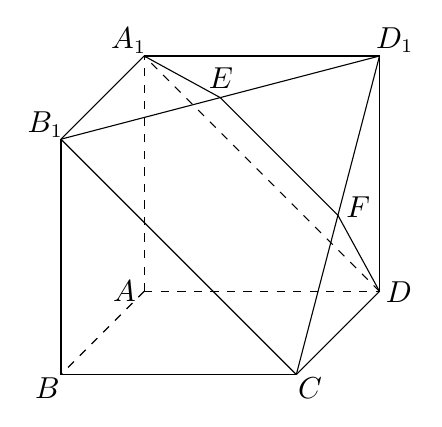
\begin{tikzpicture}[x=1pt, y=1pt,
    every node/.style={font=\fontsize{10.5pt}{12.6pt}\selectfont, inner sep=0pt}]
  % ---------- 实线 12 条（清单 §F04.2(a)）----------
  \begin{scope}[line width=0.3985pt]
    \draw (304.3280,364.6980) -- (331.8181,349.6667);   % P011 A₁E
    \draw (331.8181,349.6667) -- (374.3397,307.1451);   % P012 EF
    \draw (374.3397,307.1451) -- (389.3710,279.6550);   % P013 FD
    \draw (359.3083,249.5923) -- (389.3710,279.6550);   % P002 CD
    \draw (274.2653,249.5923) -- (359.3083,249.5923);   % P003 BC
    \draw (304.3280,364.6980) -- (274.2653,334.6353);   % P004 A₁B₁
    \draw (274.2653,334.6353) -- (389.3710,364.6980);   % P005 B₁D₁
    \draw (304.3280,364.6980) -- (389.3710,364.6980);   % P006 A₁D₁
    \draw (274.2653,249.5923) -- (274.2653,334.6353);   % P007 BB₁
    \draw (274.2653,334.6353) -- (359.3083,249.5923);   % P008 B₁C
    \draw (359.3083,249.5923) -- (389.3710,364.6980);   % P009 CD₁
    \draw (389.3710,279.6550) -- (389.3710,364.6980);   % P010 DD₁
  % ---------- 虚线 4 条（清单 §F04.2(b)）----------
    \draw[dash pattern=on 2.98883pt off 2.98883pt]
          (304.3280,279.6550) -- (389.3710,279.6550);   % P014 AD（被遮挡水平棱）
    \draw[dash pattern=on 2.98883pt off 2.98883pt]
          (389.3710,279.6550) -- (304.3280,364.6980);   % P015 DA₁（截面边）
    \draw[dash pattern=on 2.98883pt off 2.98883pt]
          (304.3280,279.6550) -- (274.2653,249.5923);   % P016 AB（被遮挡 45° 棱）
    \draw[dash pattern=on 2.98883pt off 2.98883pt]
          (304.3280,279.6550) -- (304.3280,364.6980);   % P017 AA₁（被遮挡竖直棱）
  \end{scope}
  % ---------- 字母标签（源墨迹实测中心）----------
  \node at (297.220,279.805) {$A$};    % L q19_A   清单 em 框 (297.471,278.184)
  \node at (269.329,244.611) {$B$};    % L q19_B   清单 em 框 (269.458,243.494)
  \node at (364.274,244.518) {$C$};    % L q19_C   清单 em 框 (363.835,243.494)
  \node at (396.314,279.533) {$D$};    % L q19_D   清单 em 框 (396.517,278.184)
  \node at (298.707,370.260) {$A_1$};  % L q19_A1  清单 em 框 (299.472,368.577)
  \node at (268.633,339.939) {$B_1$};  % L q19_B1  清单 em 框 (269.458,338.557)
  \node at (394.922,370.375) {$D_1$};  % L q19_D1  清单 em 框 (394.516,368.577)
  \node at (332.103,356.753) {$E$};    % L q19_E   清单 em 框 (331.486,355.568)
  \node at (381.685,310.000) {$F$};    % L q19_F   清单 em 框 (380.843,308.871)
\end{tikzpicture}
\end{center}
\nopagebreak[4]
（1） 证明：\(EF\parallel B_1C\)；

（2） 求二面角 \(E\text{-}A_1D\text{-}B_1\) 的余弦值．

\end{question}
\begin{question}
\gkti{20}设椭圆 \(E\) 的方程为 \(\dfrac{x^2}{a^2}+\dfrac{y^2}{b^2}=1\)（\(a>b>0\)），点 \(O\) 为坐标原点，点 \(A\) 的坐标为 \((a,0)\)，点 \(B\) 的坐标为 \((0,b)\)，点 \(M\) 在线段 \(AB\) 上，满足 \(|BM|=2|MA|\)，直线 \(OM\) 的斜率为 \(\dfrac{\sqrt{5}}{10}\)．

（1） 求 \(E\) 的离心率 \(e\)；

（2） 设点 \(C\) 的坐标为 \((0,-b)\)，\(N\) 为线段 \(AC\) 的中点，点 \(N\) 关于直线 \(AB\) 的对称点的纵坐标为 \(\dfrac{7}{2}\)，求 \(E\) 的方程．

\end{question}
\begin{question}
\gkti{21}设函数 \(f(x)=x^2-ax+b\)．

（1） 讨论函数 \(f(\sin x)\) 在 \(\left(-\dfrac{\pi}{2},\dfrac{\pi}{2}\right)\) 内的单调性并判断有无极值，有极值时求出极值；

（2） 记 \(f_0(x)=x^2-a_0x+b_0\)，求函数 \(|f(\sin x)-f_0(\sin x)|\) 在 \(\left[-\dfrac{\pi}{2},\dfrac{\pi}{2}\right]\) 上的最大值 \(D\)；

（3） 在 (2) 中，取 \(a_0=b_0=0\)，求 \(z=b-\dfrac{a^2}{4}\) 满足 \(D\leqslant 1\) 时的最大值．

\end{question}